\documentclass[a4paper,12pt]{article}
% \usepackage[left=1.5in, right=1in, top=1in, bottom=1in, headheight=13.6pt]{geometry}
% \usepackage[a4paper,width=150mm,top=25mm,bottom=25mm,bindingoffset=6mm]{geometry}
% \usepackage[none]{hyphenat}
% \usepackage[margin=1in]{geometry}
% \documentclass[a4paper,twoside]{book}
% \documentclass[a4paper,titlepage,openright,12pt]{MSThesis}
\usepackage[utf8]{inputenc}
\usepackage{geometry}
\usepackage{graphicx}
\usepackage{epsfig}
\usepackage[size=small,labelfont=bf,justification=centering]{caption}
\usepackage[size=footnotesize,labelfont=bf,justification=centering,skip=-10px]{subcaption}
\usepackage{booktabs}
\usepackage{float}
\usepackage{fancyhdr}
\usepackage{makeidx}
% \usepackage[nottoc,notlot,notlof]{tocbibind}
\usepackage{supertabular}
\usepackage{array}
\usepackage{setspace}
\usepackage{layout}
\usepackage{enumerate}
\usepackage{rotating}
\usepackage{moreverb}
\usepackage{tikz}
\usepackage{multirow,bigdelim}
\usepackage{makecell}
\usepackage{amsmath}
\usepackage{amsthm}
\usepackage{amssymb}
\usepackage{mathtools}
% \usepackage{captcont}
\usepackage{verbatim}
\usepackage{titlesec}
\usepackage{url}
\usepackage{listings}
\usepackage[inline]{enumitem}
\usepackage{stmaryrd}
\usepackage[hidelinks]{hyperref}
\usepackage{lipsum}
\usepackage{lscape}
\usepackage{color}
\usepackage{xr}
\usepackage{float}
\usepackage{longtable}
\usepackage{etoolbox}
\usepackage{wrapfig}
\usepackage{algorithm2e}
\usepackage{cleveref}
\usepackage{fontspec}
\usepackage{arydshln}
\usepackage[acronym,nomain]{glossaries}
%\usepackage{natbib}
\RequirePackage[numbers,square]{natbib}
\setlength{\bibsep}{0pt plus 0.3ex}
% \bibliographystyle{iitd}
% \usepackage{indentfirst}
%\usepackage{geometry}
% \usepackage[algoruled]{algorithm2e}
% \usepackage[figure,algoruled]{algorithm2e}
% \usepackage[figure,boxruled]{algorithm2e}
%\setlength{\parindent}{1.0em}
%%%%%%%%%%%%%%%%%%%%%%%%%%%%%%%%%%%%%%%%%%%%%%%%%%%%%%%%%%%%%%%%

%%%%%%%%%%%%%%%%%%%%%%%%%%%%%%%%%%%%%%%%%%%%%%%%%%

% \titlespacing\section{0pt}{5pt plus 5pt}{5pt plus 5pt}
% \titlespacing\subsection{0pt}{5pt plus 5pt}{5pt plus 5pt}
\titlespacing\subsubsection{0pt}{5pt plus 4pt minus 2pt}{5pt plus 2pt minus 2pt}

\setlength{\parskip}{1ex plus 0.5ex minus 0.2ex}
\setlength{\textheight}{8.5in}
\pagestyle{fancy}
% with this we ensure that the chapter and section
% headings are in lowercase.
\renewcommand{\bibname}{References}
% \renewcommand{\chaptermark}[1]{\markboth{#1}{}}
\renewcommand{\sectionmark}[1]{\markright{\thesection\ #1}}
\fancyhf{} % delete current setting for header and footer
%\fancyhead[LE,RO]{\bfseries\thepage}
%\fancyhead[LO]{\bfseries\rightmark}
%\fancyhead[RE]{\bfseries\leftmark}
\rhead{\fancyplain{}{\thepage}} % predefined ()
\lhead{\fancyplain{}{\rightmark}} % 1. sectionname, 1.1 subsection name etc

%\rfoot{\bfseries\thepage}
%\rfoot{\fancyplain{}{\thepage}}
% \cfoot{\em $\copyright$ 2022, Indian Institute of Technology Delhi}
\renewcommand{\headrulewidth}{0.5pt}
\renewcommand{\footrulewidth}{0.5pt}
\addtolength{\headheight}{2.5pt} % make space for the rule

\fancypagestyle{plain}{%
\fancyhead{} % get rid of headers on plain pages
\fancyfoot{}
%\rfoot{\bfseries\thepage}
% \cfoot{\em $\copyright$ 2019, Indian Institute of Technology Delhi}
\renewcommand{\headrulewidth}{0pt} % and the line
}

%% The smart version of cleardouble page.
\let\origdoublepage\cleardoublepage
\newcommand{\clearemptydoublepage}{%
  \clearpage
  {\pagestyle{empty}\origdoublepage}%
}
\usepackage{xspace}

\let\cleardoublepage\clearemptydoublepage

\setlength{\abovecaptionskip}{2px plus 2px}
\setlength{\belowcaptionskip}{2px plus 2px}

\date{}

% \addtolength{\oddsidemargin}{30pt}
% \addtolength{\evensidemargin}{-30pt}

% \titlespacing*{\chapter}{0pt}{-50pt}{20pt}
% \titleformat{\chapter}[display]{\normalfont\huge\bfseries}{\chaptertitlename\ \thechapter}{11pt}{\Huge}
\DeclareGraphicsExtensions{.pdf,.png,.jpg,.ps}
\restylefloat{figure}
\graphicspath{{./figures/}}
\sloppy\hyphenpenalty=100 \emergencystretch5em
\usetikzlibrary{arrows, quotes,shapes,positioning, calc}

\newtheorem{theorem}{Theorem}

\newenvironment{proofsketch}{\renewcommand{\proofname}{Proof Sketch}\proof}{\endproof}

\lstdefinelanguage{All}[]{C}{
  morekeywords={if,then,else,match,with,let,in,fn,type,i32,i8,bool,false,true,List,lnode,Str,clnode,u32,is,assume,assuming,do,sizeof,offsetof,typeof,addrof}
}

\lstnewenvironment{allLangEnvFoot}{\lstset{language=All,basicstyle=\footnotesize\ttfamily,mathescape=true}}{}
\lstnewenvironment{allLangEnvScript}{\lstset{language=All,basicstyle=\scriptsize\ttfamily,mathescape=true}}{}

\lstset{%
    language     = C,
    keywordstyle = \color{myastral},
    stringstyle  = \color{red},
    breaklines = false,
    commentstyle=\color{mygreen},
    keepspaces=true,
    escapeinside = ~~,
    showlines = true,
%    numbers=left,
%    numberstyle=\tiny\color{mygray},
%    numbersep=2pt,
}

\usepackage{stackengine}
\usepackage{backnaur}
\usepackage{xcolor}
\usepackage{mathtools}
\usepackage{accents}

\newcommand{\xmark}{\ding{55}}%
\newcommand{\rulesep}{\unskip\ \vrule\ }

\setlength{\textfloatsep}{6.0pt plus 1.0pt minus 1.0pt}
\setlength{\intextsep}{3.0pt plus 0.5pt minus 0.5pt}

\makeatletter
\newcommand{\oset}[3][0ex]{%
  \mathrel{\mathop{#3}\limits^{
    \vbox to#1{\kern-2\ex@
    \hbox{$\scriptstyle#2$}\vss}}}}
\makeatother

\newcommand{\toolName}{S2C}%
\newcommand{\ite}[3]{\ensuremath{#1?#2:#3}}%
\newcommand{\sumDtor}{\underline{\tt if}-\underline{\tt then}-\underline{\tt else}}%
\newcommand{\sumIs}[2]{\ensuremath{#1\ \mathrm{is}\ \cons{#2}}}%
\newcommand{\fieldPath}[2][\ensuremath{.}]{%
  \def\nextitem{\def\nextitem{#1}}% Separator
  \renewcommand*{\do}[1]{\nextitem{\field{##1}}}% How to process each item
  \docsvlist{#2}% Process list
}
\newcommand{\prodAccess}[2]{\ensuremath{#1.{\fieldPath{#2}}}}%
\newcommand{\sumIf}[1]{\underline{\tt if}\ \ensuremath{#1}}%
\newcommand{\sumThen}[1]{\underline{\tt then}\ \ensuremath{#1}}%
\newcommand{\sumElif}[1]{\underline{\tt elif}\ \ensuremath{#1}}%
\newcommand{\sumElse}[1]{\underline{\tt else}\ \ensuremath{#1}}%
\newcommand{\recursiveRelations}{recursive relations}%
\newcommand{\recursiveRelation}{recursive relation}%
\newcommand{\SpecL}{Spec}%
\newcommand{\indEq}{\ensuremath{\sim}}%
\newcommand{\indEqDepth}[1]{\ensuremath{\sim_{#1}}}%
\newcommand{\indEqUapprox}[1]{\ensuremath{\approx_{#1}}}%
\newcommand{\depthBound}[2]{\ensuremath{\Gamma_{#1}(#2)}}%
% \newcommand{\structPointer}[4]{\ensuremath{{#1} \oset{#2}{\rightarrow}_{\type{#3}} {\field{#4}}}}%
\newcommand{\structPointer}[4]{\ensuremath{{#1} \overset{#2}{\rightarrow}_{\type{#3}} {\field{#4}}}}%
\newcommand{\arrIndex}[4]{\ensuremath{#1[#2]_{#3}^{\type{#4}}}}%
\newcommand{\memRead}[3]{\ensuremath{#1[#2]_{\type{#3}}}}%
\newcommand{\memWrite}[4]{\ensuremath{#1[#2 \leftarrow #3]_{\type{#4}}}}%
\newcommand{\pointsTo}{\ensuremath{\rightsquigarrow}}%
\newcommand{\hoareTriple}[3]{\ensuremath{\{#1\}(#2)\{#3\}}}%
\newcommand{\lift}[3]{\ensuremath{{{\tt C#1}_{#2}^{\tt #3}}}}%
\newcommand{\lifted}[4]{\lift{#1}{#2}{#3}{\ensuremath{(#4)}}}%
\newcommand{\mapping}[2]{\ensuremath{#1 \! \mapsto \! #2}}%
\newcommand{\mem}{\ensuremath{\textnormal{\fontspec{STIX Two Math}\symbol{"1D55E}}}}%
\newcommand{\nonTerm}[1]{\ensuremath{\langle}#1\ensuremath{\rangle}}%
\newcommand{\term}[1]{{\tt #1}}%
\newcommand{\sv}[1]{\ensuremath{{\tt #1}_{S}}}%
\newcommand{\cv}[1]{\ensuremath{{\tt #1}_{C}}}%
\newcommand{\apc}[1]{\ensuremath{{\tt A#1}}}%
\newcommand{\bpc}[1]{\ensuremath{{\tt B#1}}}%
\newcommand{\spc}[1]{\ensuremath{{\tt S#1}}}%
\newcommand{\cpc}[1]{\ensuremath{{\tt C#1}}}%
\newcommand{\dpc}[1]{\ensuremath{{\tt D#1}}}%
\newcommand{\scpc}[2]{\ensuremath{{\tt S#1\!:\!C#2}}}%
\newcommand{\scpcinv}[2]{\ensuremath{{\phi_{\tt S#1:C#2}}}}%
\newcommand{\ddpc}[2]{\ensuremath{{\tt D#1\!:\!D#2}}}%
\newcommand{\comv}[1]{\ensuremath{{\tt #1}}}%
\newcommand{\fstv}[1]{\ensuremath{{\tt #1}^{fst}}}%
\newcommand{\sndv}[1]{\ensuremath{{\tt #1}^{snd}}}%
\newcommand{\sdef}{\ensuremath{{(\sprog{}\ {\tt def})}}}%
\newcommand{\cfits}{\ensuremath{{(\cprog{}\ {\tt fits})}}}%
\newcommand{\spath}[2][\ensuremath{{\rightarrow}}]{%
  \def\nextitem{\def\nextitem{#1}}% Separator
  \renewcommand*{\do}[1]{\nextitem{\spc{##1}}}% How to process each item
  \docsvlist{#2}% Process list
}
\newcommand{\cpath}[2][\ensuremath{{\rightarrow}}]{%
  \def\nextitem{\def\nextitem{#1}}% Separator
  \renewcommand*{\do}[1]{\nextitem{\cpc{##1}}}% How to process each item
  \docsvlist{#2}% Process list
}%
\newcommand{\dpath}[2][\ensuremath{{\rightarrow}}]{%
  \def\nextitem{\def\nextitem{#1}}% Separator
  \renewcommand*{\do}[1]{\nextitem{\dpc{##1}}}% How to process each item
  \docsvlist{#2}% Process list
}%
\newcommand{\pathpar}{\ensuremath{+}}%
\newcommand{\pathset}[2][\ensuremath{{\rightarrow}}]{%
  \def\nextitem{\def\nextitem{#1}}% Separator
  \renewcommand*{\do}[1]{\nextitem{{\tt ##1}}}% How to process each item
  \docsvlist{#2}% Process list
}
\newcommand{\scedge}[4]{\ensuremath{{\small (\scpc{#1}{#2}) \! \rightarrow \! (\scpc{#3}{#4})}}}%
\newcommand{\ddedge}[4]{\ensuremath{{\small (\ddpc{#1}{#2}) \! \rightarrow \! (\ddpc{#3}{#4})}}}%
\newcommand{\type}[1]{{\tt #1}}%
\newcommand{\ctype}[1]{{{\,\tt :\!#1}}}
\newcommand{\cons}[1]{{\tt #1}}%
\newcommand{\field}[1]{{{\tt #1}}}%
\newcommand{\mlr}[1]{{\ensuremath{\tt #1}}}%
\newcommand{\mlrf}[1]{{\ensuremath{\tt #1_1}}}%
\newcommand{\mlrs}[1]{{\ensuremath{\tt #1_{2+}}}}%
\newcommand{\lhs}{{\tt LHS}}%
\newcommand{\rhs}{{\tt RHS}}%
\newcommand{\typeof}[1]{{\tt typeof(#1)}}%
\newcommand{\sizeof}[1]{{\tt sizeof(#1)}}%
\newcommand{\offsetof}[2]{{\tt offsetof(#1,#2)}}%
\newcommand{\addrof}[1]{{\tt addrof(#1)}}%
\newcommand{\heapr}{{\ensuremath{\mathcal{H}}}}%
\newcommand{\sprog}{{\ensuremath{\mathcal{S}}}}%
\newcommand{\cprog}{{\ensuremath{\mathcal{C}}}}%
\newcommand{\dprog}{{\ensuremath{\mathcal{D}}}}%
\newcommand{\fdprog}{{\ensuremath{\mathcal{D}^{fst}}}}%
\newcommand{\sdprog}{{\ensuremath{\mathcal{D}^{snd}}}}%
\newcommand{\pre}{{\ensuremath{Pre}}}%
\newcommand{\post}{{\ensuremath{Post}}}%
\newcommand{\corrtuple}[4]{{\ensuremath{\langle #1, #2, #3, #4 \rangle}}}%
\newcommand{\ttedge}[2]{{\ensuremath{[#1 \! \rightarrow \! {\tt #2}]}}}%
\newcommand{\vtedge}[3]{{\ensuremath{[#1 \! \overset{#3}{\rightarrow} \! {\tt #2}]}}}%
\newcommand{\sumn}{\ensuremath{\circled{+}}}%
\newcommand{\prodn}{\ensuremath{\circled{\times}}}%
\newcommand{\vtse}[1]{{\ensuremath{\omega_{#1}\!}}}%
\newcommand{\oland}{\ensuremath{\underbar{\land}}}%
\newcommand{\xfer}{{\tt tf}}%
\newcommand{\execpath}{{\tt ep}}%
\newcommand{\ftrace}[1]{{\ensuremath{{\tt Ftrace}(#1)}}}%
\newcommand{\comp}[2]{{\ensuremath{{\tt Comp}_{#2}(e)}}}%
\newcommand{\retval}[1]{{\ensuremath{{\tt Retval}(#1)}}}%
\newcommand{\pathcond}[1]{{\ensuremath{{\tt Pathcond}(#1)}}}%
\newcommand{\execpaths}[3]{{\ensuremath{{\tt EP}_{#1}(#2,#3)}}}%

\newcommand{\keyword}[1]{{\ensuremath{\ \textnormal{\textbf{#1}}\ }}}%
\newcommand{\subst}[3]{{\ensuremath{\{ #2 \mapsto #3 \} #1}}}%
\newcommand{\strcat}{\ensuremath{\mathbin\Vert}}%
\newcommand{\strsep}{\ensuremath{\raisebox{0.5pt}{\underline{\phantom{x}}}}}%

\newcommand{\Tstrut}{\rule{0pt}{2.7ex}}         % = `top' strut
\newcommand{\Bstrut}{\rule[-1.2ex]{0pt}{0pt}}   % = `bottom' strut

\newcommand*{\circled}[1]{\tikz[baseline=(char.base)]{
                          \node[shape=circle,draw,inner sep=1pt] (char) {#1};}}
\newcommand*{\curved}[1]{\tikz[baseline=(char.base)]{
                      \node[shape=rounded rectangle,draw,inner sep=3pt] (char) {\footnotesize #1};}}
\newcommand*{\inv}[1]{\tikz[baseline=(char.base)]{
                      \node[shape=rounded rectangle,draw,inner sep=2pt] (char) {\scriptsize {\tt #1}};}}
\newcommand*{\pred}[1]{\fbox{\scriptsize {\tt #1}}}
\newcommand*{\tfbox}[1]{\fbox{\ensuremath{#1}}}
\newcommand*{\compacttfbox}[1]{\setlength{\fboxsep}{1pt}\fbox{\ensuremath{#1}}}

\newcommand{\invgrammar}{\ensuremath{\textnormal{\fontspec{STIX Two Math}\symbol{"1D53E}}}}%
\newcommand{\memregions}{\ensuremath{\textnormal{\fontspec{STIX Two Math}\symbol{"211D}}}}%
\newcommand{\pseudoregs}{\ensuremath{\textnormal{\fontspec{STIX Two Math}\symbol{"1D54A}}}}%
\newcommand{\typegrammar}{\ensuremath{\textnormal{\fontspec{STIX Two Math}\symbol{"1D54B}}}}%

\newcommand{\astcons}[1]{{\textcolor{myastral}{\cons{#1}}}}%
\newcommand{\olifield}[1]{{\textcolor{myolive}{\field{#1}}}}%magenta


\definecolor{myastral}{RGB}{46,116,181}
\definecolor{myolive}{named}{olive}
\definecolor{mygreen}{rgb}{0,0.6,0.2}
\definecolor{mygray}{rgb}{0.5,0.5,0.5}
\definecolor{myred}{rgb}{0.8,0,0.2}

\newcommand{\Guide}{Sorav Bansal}
\newcommand{\Auth}{Indrajit Banerjee}
\newcommand{\Entry}{(2020CSY7569)}
\newcommand{\SynopsisTitle}{Counterexample-Guided Verification of Imperative Programs Against Implementation Agnostic Functional Specification}
\newcommand{\ThesisTitle}{Counterexample-Guided Verification of Imperative Programs Against Functional Specification}
% \hypersetup{draft}
\begin{document}

\begin{titlepage}
\begin{center}
{\large {\textit{Synopsis of Thesis on}}}\\
\Large{\textbf{ \ThesisTitle}}\\
\vspace{15pt}
%\emph{A thesis submitted in partial fulfillment} \\
%\emph{of the requirements for the degree of} \\
%\vspace{15pt}
%\bfseries MASTER OF SCIENCE (RESEARCH) \\
%\vspace{20pt}
%\emph {in}\\
%\vspace{20pt}
%\bfseries Computer Science and Engineering \\
%\vspace{15pt}
\normalsize \emph {by}\\
\vspace{15pt}
\Large{\textbf{\Auth}} \\
\normalsize{\textsf{\bf \Entry}}\\
\vspace{25pt}
{\normalsize \emph {Under the guidance of}} \\
\Large{\textbf{Prof. \Guide{}}} \\
\normalsize{\textsf{\bf (Computer Science and Engineering)\\ }}
\vspace{20pt}
{\normalsize \emph {Submitted in the partial fulfillment \\of the requirements for the degree of}}\\
\vspace{10pt}
{\large \textbf{Master of Science (Research)}}\\

\vspace{15pt}
{\normalsize \emph {to the}}

\vspace{10pt}

\begin{center}

\includegraphics[scale=0.6]{chapters/figures/iitd_logo.pdf} \\
\vspace{10pt}
\end{center}

\large{\textsf{\bf Department of Computer Science and Engineering\\}}
\Large{\textsf{\bf Indian Institute of Technology Delhi\\}}
\vspace{15pt}
\large{\textsf{\bf June 2023}}
\end{center}
\end{titlepage}


% \onehalfspacing
\thispagestyle{empty}
\normalfont

% \begin{center}
\LARGE{ Certificate} 
\end{center}

\vspace{0.5in}

\hspace*{1.0em} This is to certify that the thesis titled {\bf "\ThesisTitle"},
submitted by {\bf Mr.\Auth}, to the Indian Institute of Technology, Delhi,
for award of the degree {\bf Master of Science (Research)},
is a bonafide record of the research work done by him under my supervision.
The contents of this thesis, in full or in parts, have not been submitted to any
other Institute or University for the award of any degree or diploma.

\vspace{1.5in}


{\bfseries Prof. \Guide{}} \\
{\bfseries Department of Computer Science and Engineering} \\
{\bfseries Indian Institute of Technology Delhi}\\ 

% \thispagestyle{empty}

% \begin{center}
\LARGE{Acknowledgments} 
\end{center}

\vspace{0.5in}

\setlength{\parindent}{1.0em}

I would like to sincerely thank my thesis supervisor Prof. \Guide{}
for his continuous support during my study and research.
His guidance, patience, motivation and long discussions provided a
strong platform with clear visibility and research direction.

Besides my advisor, I would like to thank my
Student Research Committee members: Prof. Sanjiva Prasad
for their insightful comments and encouragement that helped me to widen my research from various perspectives.

I am grateful to our research group members: Abhishek Rose, Shubhani at IIT Delhi for
their help and motivating discussions on various issues related to my research area.

\vspace{0.8in}


{\bfseries \Auth}





% \thispagestyle{empty}
% \setcounter{page}{1}
% \pagenumbering{roman}
% \thispagestyle{empty}

\newgeometry{right=3.5cm,left=3.5cm}
\begin{center}

\LARGE{Abstract}
\end{center}
% \vspace{-2mm}
We describe an algorithm capable of checking
equivalence of two programs that manipulate recursive
data structures such as linked lists, strings, trees
and matrices. The first program, called specification,
is written in a succint and safe functional language
with algebraic data types (ADT).
The second program, called implementation,
is written in C using arrays and pointers.
Our algorithm, based on prior work on
counterexample guided equivalence checking,
automatically searches for a bisimulation
relation between the two programs.
We formulate an algorithm for discharging
proof obligations containing relations
between recursive data structure values across
the two diverse syntaxes, which forms our first contribution.
Our proof discharge algorithm is capable
of generating falsifying counterexamples in case of
a proof failure.
As part of our proof discharge algorithm,
we formulate a program representation of values.
This allows us to reformulate proof obligations
due to the top-level equivalence check
into smaller nested equivalence checks.
Based on this algorithm,
we implement an automatic (push-bottom) equivalence checker tool named \toolName{},
which forms our second contribution.
\toolName{} is evaluated on
implementations of common string library
functions taken from popular C library implementations,
as well as,
implementations of common list, tree and matrix programs.
These implementations differ in data layout
of recursive data structures as well as
algorithmic strategies.
We demonstrate that \toolName{} is able to establish equivalence
between a single specification and all of its diverse C implementations.

% We describe an algorithm for checking equivalence of two
% programs that manipulate recursive data structures like
% lists, strings, and trees.  The first program, called
% specification,
% is written in a succinct and
% safe functional language with algebraic data types.
% The second program, called implementation,
% is written in C using arrays and pointers.
% Our algorithm automatically searches for a bisimulation
% relation between the two programs. Our
% primary contribution is an algorithm to discharge proof
% obligations that may contain expressions that relate
% (arbitrarily deep) recursive data structure values across the two
% diverse syntaxes.
% Our equivalence checker, based on this algorithm,
% can compute equivalence
% of a single abstract specification program with multiple
% C implementations that vary in their data layout and
% algorithmic strategy.

\textbf{Keywords:} \textit{Equivalence checking; Bisimulation; Recursive Data Structures; Algebraic Data Types;}

\setlength{\parindent}{1.0em}

\thispagestyle{empty}

\setcounter{tocdepth}{3}
\tableofcontents
\newpage

\setcounter{page}{1}
\pagenumbering{arabic}
\newgeometry{right=3cm,left=3cm}
\vspace{-7px}
\section{Introduction}
\label{sec:syn-intro}
\vspace{-7px}
The problem of equivalence checking between a functional specification and an
implementation written in a low level imperative language such as C
has been of major research interest
and has several important applications such as (a) program verification, where
the equivalence checker is used to verify that the C implementation
behaves according to the specification and (b) translation validation, where
the equivalence checker attempts to generate a proof of equivalence across
the transformations (and translations) performed by an optimizing compiler
and more. The verification of a C implementation against its manually written
functional specification through manually-coded refinement proofs has been
performed extensively in the seL4 microkernel \cite{seL4}.
Frameworks for program equivalence proofs have been developed in interactive
theorem provers like Coq \cite{programEquivalenceInCoq} where correlations and invariants
are manually identified during proof codification.
On the other hand, programming languages like Dafny \cite{dafny} offer automated program
reasoning for imperative languages with abstract data types such as sets and arrays.
Such languages perform automatic compile-time checks for manually-specified correctness predicates through
SMT solvers.

We present \toolName{}, an algorithm to automatically (push-button) search
for a proof of equivalence between a functional specification and its
optimized C implementation. We will demonstrate how \toolName{} is capable of
proving equivalence of multiple equivalent C implementations with vastly
different (a) data layouts (e.g. array, linked list representations of a {\em list})
and (b) algorithmic strategies (e.g. alternate algorithms, optimizations) against
a {\em single} functional specification.
This opens the possibility of regression verification \cite{strichman_regressverify,felsing14},
where \toolName{} can be used to automate verification across
software updates that change memory layouts for data structures.
We start by formulating the problem statement and define equivalence in this context.
Next, we shortly introduce bisimulation in the context of program equivalence and list our primary contributions.
\vspace{-7px}
\subsection{Problem Setting and Bisimulation}
\label{sec:syn-setting-bisimulation}
We restrict our attention to programs that construct, read, and write
to recursive data structures. In languages like C, pointer and array based
implementations of these data-structures are prone to safety and liveness bugs.
Similar recursive data structures are also available in safer functional languages like Haskell,
where algebraic data types (ADTs) \cite{hope} ensure several safety properties.
We define a minimal functional language, called \SpecL{}, that enables the safe
and succinct specification of programs manipulating and traversing recursive data structures.
\SpecL{} is equipped with ADTs as well as boolean and bitvector (\type{i<N>}) types.

\begin{figure}[H]
\begin{tabular}{cc}
\begin{subfigure}[b]{0.565\textwidth}
\begin{center}
\begin{allLangEnvScript}
~{\tiny \textcolor{mygray}{A0:}}~ type List = LNil | LCons (val:i32, tail:List).
~{\tiny \textcolor{mygray}{A1:}}~
~{\tiny \textcolor{mygray}{A2:}}~ fn mk_list_impl (n:i32) (i:i32) (l:List):List=
~{\tiny \textcolor{mygray}{A3:}}~    if ${\tt i \geq_u n}$ then l
~{\tiny \textcolor{mygray}{A4:}}~    else make_list_impl(n, i+${\tt 1_{i32}}$, LCons(i, l)).
~{\tiny \textcolor{mygray}{A5:}}~
~{\tiny \textcolor{mygray}{A6:}}~ fn mk_list (n:i32):List=
~{\tiny \textcolor{mygray}{A7:}}~    mk_list_impl(n, ${\tt 0_{i32}}$, LNil).
\end{allLangEnvScript}
\end{center}
\caption{\label{fig:llAllocSpec}Spec Program}
\end{subfigure}%
&
\begin{subfigure}[b]{0.435\textwidth}
\begin{center}
\begin{allLangEnvScript}
~{\tiny \textcolor{mygray}{S0:}}~ List mk_list (i32 n) {
~{\tiny \textcolor{mygray}{S1:}}~   List l $\coloneqq$ LNil;
~{\tiny \textcolor{mygray}{S2:}}~   i32  i $\coloneqq$ ${\tt 0_{i32}}$;
~{\tiny \textcolor{mygray}{S3:}}~   while ${\tt \neg (i \geq_{u} n)}$:
~{\tiny \textcolor{mygray}{S4:}}~     l $\coloneqq$ LCons(i, l);
~{\tiny \textcolor{mygray}{S5:}}~     i $\coloneqq$ i + ${\tt 1_{i32}}$;
~{\tiny \textcolor{mygray}{S6:}}~   return l;
~{\tiny \textcolor{mygray}{SE:}}~ }
\end{allLangEnvScript}
\end{center}
\caption{\label{fig:llAllocSpecIR}(Abstracted) Spec IR}
\end{subfigure}%
\\
\begin{subfigure}[b]{0.565\textwidth}
\begin{center}
\begin{allLangEnvScript}
~{\tiny \textcolor{mygray}{B0: }}~ typedef struct lnode {
~{\tiny \textcolor{mygray}{B1: }}~   unsigned val; struct lnode* next; } lnode;
~{\tiny \textcolor{mygray}{B2: }}~ 
~{\tiny \textcolor{mygray}{B3: }}~ lnode* mk_list(unsigned n) {
~{\tiny \textcolor{mygray}{B4: }}~   lnode* l = NULL;
~{\tiny \textcolor{mygray}{B5: }}~   for (unsigned i = 0; i < n; ++i) {                       $\phantom{\mem{} \coloneqq {\tt \mem{}[ \& (\structPointer{\tt p}{\mem{}}{lnode}{val}) \leftarrow i]_{i32}};}$
~{\tiny \textcolor{mygray}{B6: }}~     lnode* p = malloc(sizeof lnode);                       $\phantom{\mem{} \coloneqq {\tt \mem{}[\&  (\structPointer{\tt p}{\mem{}}{lnode}{next}) \leftarrow l]_{i32}};}$
~{\tiny \textcolor{mygray}{B7: }}~     p$\rightarrow$val = i; p$\rightarrow$next = l; l = p;
~{\tiny \textcolor{mygray}{B8: }}~   }
~{\tiny \textcolor{mygray}{B9: }}~   return l;
~{\tiny \textcolor{mygray}{B10:}}~ }
\end{allLangEnvScript}
\end{center}
\caption{\label{fig:llAllocC}C Program with {\tt malloc()}}
\end{subfigure}%
&
\begin{subfigure}[b]{0.435\textwidth}
\begin{center}
\begin{allLangEnvScript}
~{\tiny \textcolor{mygray}{C0:}}~ i32 mk_list (i32 n) {
~{\tiny \textcolor{mygray}{C1:}}~   i32 l $\coloneqq$ ${\tt 0_{i32}}$;
~{\tiny \textcolor{mygray}{C2:}}~   i32 i $\coloneqq$ ${\tt 0_{i32}}$;
~{\tiny \textcolor{mygray}{C3:}}~   while ${\tt i <_{u} n}$:
~{\tiny \textcolor{mygray}{C4:}}~     i32 p $\coloneqq$ malloc$_{\tt C4}$(sizeof lnode);
~{\tiny \textcolor{mygray}{C5:}}~     $\mem{}$ $\coloneqq$ ${\tt \mem{}[ \& (\structPointer{\tt p}{\mem{}}{lnode}{val}) \leftarrow i]_{i32}}$;
~{\tiny \textcolor{mygray}{C6:}}~     $\mem{}$ $\coloneqq$ ${\tt \mem{}[\&  (\structPointer{\tt p}{\mem{}}{lnode}{next}) \leftarrow l]_{i32}}$;
~{\tiny \textcolor{mygray}{C7:}}~     l $\coloneqq$ p;
~{\tiny \textcolor{mygray}{C8:}}~     i $\coloneqq$ i + ${\tt 1_{i32}}$;
~{\tiny \textcolor{mygray}{C9:}}~   return l;
~{\tiny \textcolor{mygray}{CE:}}~ }
\end{allLangEnvScript}
\end{center}
\caption{\label{fig:llAllocCIR}(Abstracted) C IR}
\end{subfigure}%
\\
\end{tabular}
\caption{\label{fig:llAllocSpecAndC}Spec and C programs for constructing a linked list along with their corresponding abstracted intermediate representations.}
\end{figure}

\Cref{fig:llAllocSpec,fig:llAllocC} show the construction of lists in \SpecL{} and C respectively.
The inputs to a \SpecL{} procedure are its well-typed arguments, which may include recursive data structure
values. The inputs to a C procedure are its explicit arguments and the implicit state of program memory
at procedure entry. We lower both \SpecL{} and C programs to a
Three-Address-Code (3AC) style intermediate representation (IR)
as shown in \cref{fig:llAllocSpecIR,fig:llAllocCIR}. For a \SpecL{} program,
(a) all tail-recursive calls are converted to loops in IR while non-tail calls are preserved and
(b) {\tt match} statements are lowered to equivalent \sumDtor{} conditionals.
For a C program, (a) the sizes and memory layouts of both scalar (e.g., {\tt int})
and compound (e.g., {\tt struct}) types are concretized in IR and
(b) all allocation functions (e.g., {\tt malloc}) are annotated with their
call-site i.e. IR PC (e.g., {\tt malloc$_\cpc{4}$} in \cref{fig:llAllocCIR}).

\subsubsection{Equivalence Definition}
\label{sec:syn-equivalence}
\toolName{} computes equivalence between the IRs of the \SpecL{} and C sources respectively.
Henceforth, we will omit the sources and continue to refer to the IRs as \SpecL{} and C directly.
Given (1) a \SpecL{} program specification $S$, (2) a C implementation $C$,
(3) a precondition $Pre$ that relates the inputs {\tt Input}$_S$ and {\tt Input}$_C$ to $S$ and $C$
respectively, and (4) a postcondition $Post$ that relates the final outputs {\tt Output}$_S$
and {\tt Output}$_C$ of $S$ and $C$ respectively:
$S$ and $C$ are {\em equivalent} if for all possible inputs \sv{Input} and \cv{Input} such that
$Pre(\sv{Input},\cv{Input})$ holds,
$S$'s execution is well-defined on \sv{Input} i.e. \sdef{}, {\em and} C's
memory allocation requests during its execution on \cv{Input} are successful i.e. \cfits{},
then both programs $S$ and $C$ produce outputs
that satisfy $Post$.
$$
Pre(\sv{Input},\cv{Input}) \land \sdef{} \land \cfits{} \Rightarrow Post(\sv{Output},\cv{Output})
$$

\begin{figure}[]
\begin{tabular}{ccc}
\begin{subfigure}[b]{0.27\textwidth}
\begin{center}
{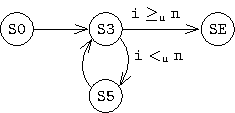
\includegraphics[scale=1]{chapters/figures/figMallocSpecCfg.pdf}}
\vspace{2pt}
\end{center}
\caption{\label{fig:llAllocSpecIRCFG}CFG of \SpecL{} Program}
\end{subfigure}%
&
\begin{subfigure}[b]{0.27\textwidth}
\begin{center}
{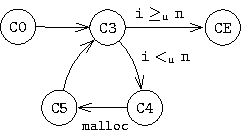
\includegraphics[scale=0.95]{chapters/figures/figMallocCCfg.pdf}}
\vspace{7pt}
\end{center}
\caption{\label{fig:llAllocCCFG}CFG of C Program}
\end{subfigure}%
&
\begin{subfigure}[b]{0.36\textwidth}
\begin{center}
{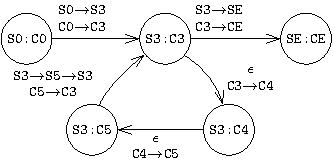
\includegraphics[scale=1]{chapters/figures/figMallocProductCfg.pdf}}
\end{center}
\caption{\label{fig:llAllocProductCFG}CFG of Product Program}
\end{subfigure}%
\\
\end{tabular}
\caption{\label{fig:mallocSpecCFGAndCCFGAndProductCFG}CFG representation for Spec and C IRs shown in \cref{fig:llAllocSpecIR,fig:llAllocCIR}.\\ \Cref{fig:llAllocProductCFG} shows a product-CFG between the CFGs in \cref{fig:llAllocSpecIRCFG,fig:llAllocCCFG}.}
\end{figure}

\begin{table}[H]
\begin{center}
\caption{\label{tab:llproductInv}Node Invariants for Product-CFG in \cref{fig:llAllocProductCFG}}
\setlength{\belowcaptionskip}{-30pt}
\begin{footnotesize}
\begin{tabular}{|c|llll|}
\hline
\tt PC-Pair & \multicolumn{4}{c|} {\tt Invariants} \\
\hline
\hline
${\tt (S0:C0)}$ &
\multicolumn{4}{l|} {\Tstrut ${\tt { \circled{P}}\  n_{S}=n_{C}}$} \\
${\tt (S3:C3)}$ &
\Tstrut  ${\tt {\scriptsize \circled{I1}}\  n_{S}=n_{C}}$ & ${\tt {\scriptsize \circled{I2}}\  i_{S}=i_{C}}$ & ${\tt {\scriptsize \circled{I3}}\  i_{S} \leq_{u} n_{S}}$ & ${\tt {\scriptsize \circled{I4}}\  l_{S}\indEq{}Clist^{lnode}_{m}(l_{C})}$ \\
${\tt (S3:C4)\ (S3:C5)}$ &
\Tstrut  ${\tt {\scriptsize \circled{I5}}\  n_{S}=n_{C}}$ & ${\tt {\scriptsize \circled{I6}}\  i_{S}=i_{C}}$ & ${\tt {\scriptsize \circled{I7}}\  i_{S} <_{u} n_{S}}$ & ${\tt {\scriptsize \circled{I8}}\  l_{S}\indEq{}Clist^{lnode}_{m}(l_{C})}$ \\
${\tt (SE:CE)}$ &
\multicolumn{4}{l|} {\Tstrut  ${\tt {\circled{E}}\  ret_{S}\indEq{}Clist^{lnode}_{m}(ret_{C})}$} \\
\hline
\end{tabular}
\end{footnotesize}
\end{center}
\end{table}

\vspace{-5px}
\Cref{fig:llAllocSpecIRCFG,fig:llAllocCCFG} show the Control-Flow Graph (CFG) representation
of the \SpecL{} and C programs in \cref{fig:llAllocSpecIR,fig:llAllocCIR} respectively.
Each node represent a PC location of its corresponding program, and each edge represent
transitions between PCs through instruction execution. For brevity, we often represent
a sequence of instructions with a single edge, e.g., in \cref{fig:llAllocCCFG}, the edge
\cpath{5,3} represents the path \cpath{5,6,7,8,3}.
A control-flow edge is associated with an {\em edge condition} (the condition under which that edge is taken),
a {\em transfer function} (how the program state is mutated if that edge is taken),
and a {\em UB assumption} (what condition should be true for the program
execution to be well-defined across this edge).

\subsubsection{Bisimulation Relation}
\label{sec:syn-bisim}
We construct a {\em bisimulation relation} to identify equivalence between two programs.
A bisimulation relation correlates the transitions of $S$ and $C$ in lockstep, such that the
lockstep execution ensures identical observable behavior.
A bisimulation relation between two programs can be represented using a {\em product program}
\cite{covac} and the CFG representation of a product program is called a {\em product-CFG}.
\Cref{fig:llAllocProductCFG} shows a product-CFG, that encodes the lockstep execution
(bisimulation relation) between the CFGs in \cref{fig:llAllocSpecIRCFG,fig:llAllocCCFG}.

\Cref{tab:llproductInv} shows the precondition (labeled \circled{\small P}),
inductive invariants (labeled \circled{\small I}) and postcondition (labeled \circled{\small E})
for the product-CFG in \cref{fig:llAllocProductCFG}. The precondition and postcondition are
provided manually by the user while the intermediate inductive invariants are inferred automatically.
The invariant labeled \circled{\small I4} is an example of a {\em \recursiveRelation{}} and represents
equality between the \SpecL{} \type{List} variable \sv{l} and the \type{List} represented by
chasing \type{lnode} pointers starting at \cv{l}.
Semantically $l_1\indEq{}l_2$ and $l_1=l_2$ are equivalent, `\indEq{}' simply emphasizes the
fact that $l_1$ and $l_2$ are values of (possibly recursive) ADT types.
\lifted{list}{\mem{}}{lnode}{p} is called a {\em lifting constructor} that {\em lifts}
the C pointer value {\tt p} (pointing to an object of type \type{struct lnode}) and the C
memory state \mem{} to a (possibly infinite in case of a circular list)
\SpecL{} \type{List} value, and is defined as follows:
\begin{equation}
\label{eqn:clist}
\begin{split}
U_C:\ &\lifted{list}{\mem{}}{lnode}{p \ctype{i32}} = \sumIf{p=0} \ \sumThen{\cons{LNil}} \\ & \qquad\qquad\ \ \ \sumElse{\cons{LCons}(\structPointer{p}{\mem{}}{lnode}{val}, \lifted{list}{\mem{}}{lnode}{\structPointer{p}{\mem{}}{lnode}{next}})}
\end{split}
\end{equation}
The iterative construction of the product-CFG along with inference of inductive invariants at its nodes are based on
prior work \cite{oopsla20} and discussed briefly in \cref{sec:syn-contribs}. Given a product-CFG
and inferred invariants, the equivalence checker attempts to prove each inductive invariant and
postcondition under the appropriate preconditions for each edge in the product-CFG. These proof
obligations are expressed as relational Hoare triples \cite{relationalHoareLogic,hoareTriple}
and lowered to a first order logic predicate using weakest precondition predicate transformer.
For example, \hoareTriple{\phi_s}{\sv{\rho},\cv{\rho}}{\phi_d}
represents the Hoare triple where $\phi_s$ and $\phi_d$ represents the pre- and postconditions
and (\sv{\rho},\cv{\rho}) represents a product-CFG edge correlating the paths \sv{\rho} and \cv{\rho}
in $S$ and $C$ respectively. The above Hoare triple lowers to the following predicate:
\begin{equation}
\label{eqn:firstOrderFormula}
(\phi_s \land pathcond_{\sv{\rho}} \land pathcond_{\cv{\rho}} \land ubfree_{\sv{\rho}}) \Rightarrow {\tt WP}_{{\sv{\rho},\cv{\rho}}}(\phi_d)
\end{equation}
We will use `\lhs{}' and `\rhs{}' to refer to the antecedent and consequent of the
implication operator `$\Rightarrow$' in \cref{eqn:firstOrderFormula}.
These proof obligations often contains \recursiveRelations{} encoding equality between
arbitrarily-deep recursively data structure values of $S$ and $C$ respectively.
The handling of these proof obligations is a major challenge and forms our primary
contribution as discussed next in \cref{sec:syn-contribs}.
\vspace{-5px}
\subsection{Our Contributions}
\label{sec:syn-contribs}
As previously discussed in \cref{sec:syn-bisim}, showing equivalence through a bisimulation proof
requires three major steps:
\circled{\small 1} An algorithm for construction of a product-CFG by correlating
program executions across the \SpecL{} and C programs respectively,
\circled{\small 2} An algorithm for identification of inductive invariants at correlated PCs and
\circled{\small 3} A proof discharge algorithm for discharging proof obligations containing \recursiveRelations{}.
Our major contributions are as follows:

\begin{itemize}
\setlength{\itemsep}{0px}
\item Proof Discharge Algorithm: Discharging proof obligations (\circled{\small 3})
involving \recursiveRelations{} is rather challenging and forms our primary contribution.
We describe a {\em sound} proof discharge algorithm capable of tackling proof obligations involving
\recursiveRelations{} using off-the-shelf SMT solvers. Our proof discharge algorithm is also capable of
reconstruction of counterexamples for the original proof query from models returned by the individual SMT queries.
These counterexamples are the backbone of counterexample-guided algorithms for
\circled{\small 1} and \circled{\small 2} steps. As part of our proof discharge procedure,
we reformulate equality of values (i.e. \recursiveRelations{}) as equivalence of their corresponding programs
and discharge these proof queries using a nested (albeit much simpler) bisimulation check.

\item Spec-to-C Equivalence Checker Tool: Our second contribution is \toolName{}, an equivalence checker tool
capable of proving equivalence between a \SpecL{} and a C program automatically. \toolName{} is based on
the Counter tool\cite{oopsla20} and uses modified versions of (a) counterexample-guided correlation algorithm for
incremental construction of a product-CFG and (b) counterexample-guided invariant inference algorithm
for inference of inductive invariants at correlated PCs in the (partially constructed) product-CFG.
\toolName{} discharges required verification conditions (i.e. proof obligations) using our Proof Discharge Algorithm.
\end{itemize}
\vspace{-5px}
\Cref{sec:syn-examples} walks through our proof discharge algorithm by demonstrating each of its
components using examples. We evaluate our equivalence checking tool \toolName{} in \cref{sec:syn-eval}.
Finally, \cref{sec:syn-limitations} gives an overview of its limitations and \cref{sec:syn-conclusion} concludes our discussion.
\section{Proof Discharge Algorithm through Examples}
\label{sec:syn-examples}
This section demonstrates our proof discharge algorithm through example programs
that construct and traverse a linked list respectively. Our equivalence checker has the property
that it is safe to return false (i.e. disproven) for all proof obligations. Keeping this in mind,
our proof discharge algorithm is designed to be {\em sound} i.e. (a) whenever it evaluates a proof obligation
to true (i.e. proven), the actual proof obligation must also be proven and (b) whenever it returns
false with a set of counterexamples, the counterexamples must falsify the actual proof obligation.
However, it is possible for our proof discharge algorithm to return false (without a counterexample)
even if the actual proof obligation is true.
Our equivalence checking algorithm also ensures that, for an invariant
$\phi_s=({\tt \phi^{1}_s \land \phi^{2}_s \land ... \land \phi^{k}_s})$,
at any node $s$ of a product-CFG,
if a \recursiveRelation{} appears in $\phi_s$, it
must be one of $\phi^{1}_s$, $\phi^{2}_s$, ..., or $\phi^{k}_s$. We call
this the {\em conjunctive \recursiveRelation{}} property of an invariant $\phi_s$.

A proof obligation
$\hoareTriple{\phi_s}{e}{\phi_d}$, where $e=(\rho_S,\rho_C)$,
gets lowered using
${\tt WP}_{e}(\phi_d)$ (as shown in \cref{eqn:firstOrderFormula}) to a first-order logic formula of the following form:
\vspace{-5px}
\begin{equation}
\label{eqn:proofObligationShape}
(\eta^{l}_1 \land \eta^{l}_2 \land ... \land \eta^{l}_m) \Rightarrow (\eta^{r}_1 \land \eta^{r}_2 \land ... \land \eta^{r}_n)
\vspace{-5px}
\end{equation}
% In this formula,
% the {\tt LHS} and {\tt RHS} are
% written as conjunctions of $\eta^{l}_i$ and $\eta^{r}_j$ respectively (for $1\leq i\leq m$, $1\leq j\leq n$).
% Each $\eta^{r}_j$ relation is obtained from
% ${\tt WP}_{e}(\phi^{j}_d)$, where $\phi_d=({\tt \phi^{1}_d \land \phi^{2}_d \land ... \land \phi^{n}_d})$.
Thus, due to the conjunctive \recursiveRelation{} property of $\phi_s$ and $\phi_d$, any
\recursiveRelation{} in \cref{eqn:proofObligationShape} must appear as
one of $\eta^{l}_i$ or $\eta^{r}_j$.
To simplify proof obligation discharge,
we break a first-order logic proof obligation $P$ of the form in \cref{eqn:proofObligationShape}
into multiple smaller proof obligations
of the form
$P_j:(\lhs{} \Rightarrow{\tt \eta^{r}_j})$, for $j=1..n$. Each proof obligation
$P_j$ is then discharged separately.  We call this conversion from
a bigger query to multiple smaller queries, {\em \rhs{}-breaking}.

%We say that two relations $\eta_1$ and $\eta_2$ {\em interfere}, written
%$\eta_1 \interfere{} \eta_2$,
%iff the intersection
%of the sets of free variables mentioned in $\eta_1$ and $\eta_2$
%is non-empty.  For example, $a\indEq{}b$ and $c\indEq{}d$
%do not interfere, but $a\indEq{}b$ and $c\indEq{}{\tt LCons}(0,b)$ interfere.
%
%In a proof obligation of the form in \cref{eqn:proofObligationShape},
%two relations $\eta_1$ and $\eta_2$ {\em transitively interfere} iff
%there exists a relation $\eta_3$ in the proof
%obligation such that $\eta_1\interfere{}\eta_3$ and $\eta_3\interfere{}\eta_2$.
%This notion of transitive interference can be lifted
%to Hoare triples: in a proof obligation $\{\phi_s\}(e)\{\phi_d\}$,
%where $\phi_{s}=\phi^{1}_s\land...\phi^{k}_{s}$ and $\phi_{d}=\phi^{1}_d\land...\phi^{n}_{d}$,
%an {\tt LHS} conjunctive clause $\phi^{i}_s$ transitively
%interferes with an {\tt RHS} conjunctive clause $\phi^{j}_d$ iff
%$\phi^{i}_s$
%transitively interferes with ${\tt WP}_{e}(\phi^{j}_d)$ in
%the lowered first-order logic formula.

%We provide a sound (but imprecise) proof discharge
%algorithm that converts
%a proof obligation generated by our equivalence
%checker into a series of SMT queries.
%Our
%algorithm begins
%by categorizing a proof obligation
%into three categories, and each
%category is discussed separately
%in subsequent sections.  These categories are created
%based on an iterative unrolling and unification
%procedure, which we describe next.
%We use an unroll parameter $k$ for
%our categorization.
\subsection[Categorization of Proof Obligations]{Categorization of Proof Obligations based on \\Decomposition of Recursive Relations}
\label{sec:syn-cat-decomp}
Before diving into the proof discharge algorithm, we start with a key procedure in our proof discharge algorithm called `decomposition of \recursiveRelations{}'.
\vspace{-5px}
\begin{equation}
\label{eqn:specDeconstruct}
U_S: l = \sumIf{\sumIs{l}{LNil}} \  \sumThen{\cons{LNil}} \  \sumElse{\cons{LCons}(\prodAccess{l}{val}, \prodAccess{l}{next})}
\vspace{-5px}
\end{equation}
Firstly, an expression $e$ whose top-level operator is a lifting constructor, (e.g., \lifted{list}{\mem{}}{lnode}{\cv{l}}), is called a {\em lifted expression}.
A \recursiveRelation{} of the form $l_1 \indEq{} l_2$ can be {\em decomposed} into an
equivalent set of {\em decomposition clauses}, each of the form $(P\! \rightarrow\! A\! =\! B)$ or $(P\! \rightarrow\! A\! \indEq{}\! B)$.
The primary algorithm behind decomposition is an iterative unification and rewriting procedure under a set of rewriting rules $E$.
$E$ allows rewriting of lifted expressions by their corresponding definitions (e.g., \cref{eqn:clist}),
and expansion of ADT variables using \sumDtor{} as shown in \cref{eqn:specDeconstruct}.
Unification proceeds by (a) recursively unifying the structures created by the top-level ADT constructors (e.g., \cons{LCons}) as well as the \sumDtor{}
operator and (b) rewriting the top-level expressions using rules in $E$, as necessary.
For example, \sumIf{c_1} \ \sumThen{\cons{LNil}} \ \sumElse{\cons{LCons}(0,l_1)} \indEq{} \sumIf{c_2} \ \sumThen{\cons{LNil}} \ \sumElse{\cons{LCons}(i, \lifted{list}{\mem{}}{lnode}{l_2})}
decomposes into $\bigwedge\{c_1=c_2, (\neg c_1 \land \neg c_2) \rightarrow 0=i, (\neg c_1 \land \neg c_2) \rightarrow l_1 \indEq{} \lifted{list}{\mem{}}{lnode}{l_2} \}$.
Similarly, the decomposition of $l_1\indEq{} \cons{LCons}(42, \lifted{list}{\mem{}}{lnode}{l_2})$ is given by
$\bigwedge \{\sumIs{l_1}{LCons}, (\sumIs{l_1}{LCons}) \rightarrow (\prodAccess{l_1}{val}=42), (\sumIs{l_1}{LCons}) \rightarrow (\prodAccess{l_1}{next} \indEq{} \lifted{list}{\mem{}}{lnode}{l_2}) \}$.
The {\em decomposition} of an expression $e$ is found by decomposing each \recursiveRelation{} in $e$.

We {\em unroll a \recursiveRelation{} $l_1 \indEq{} l_2$ with respect to $E$} by rewriting the top-level expressions $l_1$ and $l_2$ through $E$ (if possible) and decomposing it.
We {\em unroll an expression $e$} by unrolling each \recursiveRelation{} in $e$ with respect to $E$.
More generally, the $k$-unrolling of $e$ is found by unrolling the $(k-1)$-unrolling of $e$ recursively.
For a first order logic proof obligation $P:\lhs{} \Rightarrow \rhs{}$, we identify its $k$-unrolling (for a fixed unrolling parameter $k$).
After unrolling, we eliminate those decomposition clauses $(P_i\! \rightarrow\! X_i)$ whose $P_i$ evaluates to false under the \lhs{} ignoring all \recursiveRelations{}.
For example, the one-unrolling of $P: \lhs{} \Rightarrow l \indEq{} \lifted{list}{\mem{}}{lnode}{0}$, after elimination, yields $P': \lhs{} \Rightarrow \sumIs{l}{LNil}$.
We categorize a proof obligation $P: \lhs{} \Rightarrow \rhs{}$ based on this $k$-unrolled form of decomposition of $P$ as follows:
\vspace{-5px}
\begin{itemize}
\setlength{\itemsep}{-3px}
\item Type I: $k$-unrolling of $P$ does not contain \recursiveRelations{}
\item Type II: $k$-unrolling of $P$ contains \recursiveRelations{} only in the \lhs{}
\item Type III: $k$-unrolling of $P$ contains \recursiveRelations{} in the \rhs{}
\end{itemize}
\vspace{-10px}
Next, we briefly describe the key ideas for each of the three types of proof obligations in \cref{sec:syn-cat1,sec:syn-cat2,sec:syn-cat3}.

\begin{figure}
\begin{tabular}{cc}
\begin{subfigure}[b]{0.45\textwidth}
\begin{center}
\begin{allLangEnvFoot}
~{\scriptsize \textcolor{mygray}{   }}~   
~{\scriptsize \textcolor{mygray}{S0:}}~ i32 sum_list (List l) {
~{\scriptsize \textcolor{mygray}{S1:}}~   i32 sum $\coloneqq$ ${\tt 0_{i32}}$;
~{\scriptsize \textcolor{mygray}{S2:}}~   while $\neg$(l is LNil):
~{\scriptsize \textcolor{mygray}{S3:}}~     // (l is LCons);
~{\scriptsize \textcolor{mygray}{S4:}}~     sum $\coloneqq$ sum + l.val;
~{\scriptsize \textcolor{mygray}{S5:}}~     l   $\coloneqq$ l.next;
~{\scriptsize \textcolor{mygray}{S6:}}~   return sum;
~{\scriptsize \textcolor{mygray}{SE:}}~ }
\end{allLangEnvFoot}
\end{center}
\caption{\label{fig:llTraverseSpecIR}(Abstracted) Spec IR}
\end{subfigure}%
&
\begin{subfigure}[b]{0.55\textwidth}
\begin{center}
\begin{allLangEnvFoot}
~{\scriptsize \textcolor{mygray}{\ \ \ }}~ unsigned sum_list (lnode* l);
~{\scriptsize \textcolor{mygray}{C0:}}~ i32 sum_list (i32 l) {
~{\scriptsize \textcolor{mygray}{C1:}}~   i32 sum $\coloneqq$ ${\tt 0_{i32}}$;
~{\scriptsize \textcolor{mygray}{C2:}}~   while ${\tt l \neq 0_{i32}}$:
~{\scriptsize \textcolor{mygray}{C3:}}~     sum $\coloneqq$ sum + $\structPointer{\tt l}{\mem{}}{lnode}{val}$;
~{\scriptsize \textcolor{mygray}{C4:}}~     l   $\coloneqq$ $\structPointer{\tt l}{\mem{}}{lnode}{next}$;
~{\scriptsize \textcolor{mygray}{C5:}}~   return sum;
~{\scriptsize \textcolor{mygray}{CE:}}~ }
\end{allLangEnvFoot}
\end{center}
\caption{\label{fig:llTraverseCIR}(Abstracted) C IR}
\end{subfigure}%
\\
\end{tabular}
\caption{\label{fig:llTraverseSpecIRAndCIR}IRs for the \SpecL{} and C Programs in \cref{fig:llTraverseSpec,fig:llTraverseC} respectively.}
\end{figure}

\vspace{-10px}
\subsection{Handling Type I Proof Obligations}
\label{sec:syn-cat1}
In \cref{fig:llAllocProductCFG}, consider a proof obligation generated
across the product-CFG edge \scedge{0}{0}{3}{3}
while checking if the {\circled{\footnotesize I4}} invariant in \cref{tab:llproductInv} holds at (\scpc{3}{3}):
\hoareTriple{\scpcinv{0}{0}}{\spath{0,3},\cpath{0,3}}{\sv{l} \indEq{} \lifted{list}{\mem{}}{lnode}{\cv{l}}}.
The precondition $\scpcinv{0}{0} \equiv (\sv{n} = \cv{n})$ does not contain a \recursiveRelation{}.
When lowered to first-order logic through {\tt WP}$_{\spath{0,3},\cpath{0,3}}$, this translates to
$\sv{n} = \cv{n} \Rightarrow \cons{LNil} \indEq{} \lifted{list}{\mem{}}{lnode}{0}$.
Here, \cons{LNil} is obtained for \sv{l} and {\tt 0} (null) is obtained for \cv{l}.
The one-unrolled form of this proof obligation yields
$\sv{n} = \cv{n} \Rightarrow true$ which trivially resolves to true.

Consider the following example of a proof obligation:
\hoareTriple{\scpcinv{0}{0}}{\spath{0,3,5,3}, \\ \cpath{0,3}}{\sv{l} \indEq{} \lifted{list}{\mem{}}{lnode}{\cv{l}}}.
Notice, we have changed the path in $S$ to \spath{0,3,5,3} here.
In this case, the corresponding first-order logic formula evaluates to:
$\sv{n} = \cv{n} \land 0 <_u \sv{n} \Rightarrow \cons{LCons}(0, \cons{LNil}) \indEq{} \lifted{list}{\mem{}}{lnode}{0}$.
One-unrolling of this proof obligation decomposes \rhs{} into false due to
failed unification of \cons{LCons} and \cons{LNil}.
The proof obligation is further discharged using an SMT solver
which provides a counterexample (model) that evaluates the
formula to false. For example, the counterexample $\{ \mapping{\sv{n}}{42}, \mapping{\cv{n}}{42} \}$
evaluates this formula to false.
% because
% this fails to unify (during decomposition), it evaluates to false.
% When a
% proof obligation evaluates to false, the SMT solver
% provides a counterexample (model) that evaluates the condition
% to false.  For example, the counterexample {\tt n$_S$=n$_C$=42}
% evaluates this condition to false.
These counterexamples
assist in faster convergence
of our invariant inference and correlation search procedures as part of the \toolName{} tool.
% Thus, we unify the structure and
% values of the \SpecL{} objects on both sides of
% the $\sim$ operator (after $k$ unrollings), and discharge the resulting
% proof obligations (that relate bitvector and array values) using an SMT solver.
% Please refer to {\tt Chapter \ThesisChapterAlgo{}} of the thesis for
% the intricacies of (a) translation of the formlua to SMT logic and (b) reconstruction
% of counterexamples from the models returned by the SMT solver.
% Assuming a capable enough SMT solver,
% all proof obligations in Type I can be discharged precisely, i.e.,
% we can always decide whether $P$ evaluates to true or false. If it
% evaluates to false, we also obtain a counterexample.

\begin{figure}
\begin{tabular}{cc}
\begin{subfigure}[b]{0.45\textwidth}
\begin{center}
{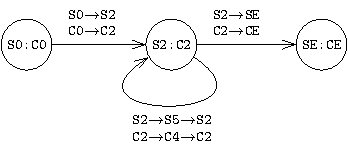
\includegraphics[scale=1.1]{chapters/figures/figSumListProductCfg.pdf}}
\end{center}
\caption{\label{fig:llTraverseProduct}Product-CFG}
\end{subfigure}%
&
\begin{subfigure}[b]{0.55\textwidth}
\begin{center}
\begin{footnotesize}
\begin{tabular}{|c|l|}
\hline
{\bf PC-Pair} & \multicolumn{1}{c|} {\bf Invariants} \\
\hline
\hline
(\scpc{0}{0}) &
\Tstrut $\circled{P}\  \sv{l} \indEq{} \lifted{list}{\mem{}}{lnode}{\cv{l}}$ \\
\multirow{2}{*}{(\scpc{2}{2})} &
\Tstrut $\circled{\scriptsize I1}\  \sv{l} \indEq{} \lifted{list}{\mem{}}{lnode}{\cv{l}}$ \\ &
\Tstrut $\circled{\scriptsize I2}\  \sv{sum} = \cv{sum}$ \\
(\scpc{E}{E}) &
\Tstrut $\circled{\scriptsize E}\  \sv{ret} = \cv{ret}$ \\
\hline
\end{tabular}
\end{footnotesize}
\vspace{13px}
\end{center}
\caption{\label{fig:llTraverseProductInv}Node Invariants of the Product-CFG}
\end{subfigure}%
\\
\end{tabular}
\caption{\label{fig:llTraverseProductCFGInvs} Product-CFG between the IRs in \cref{fig:llTraverseSpecIR,fig:llTraverseCIR}. The inductive invariants of the Product-CFG are given in \cref{fig:llTraverseProductInv}.}
\end{figure}


\subsection{Handling Type II Proof Obligations}
\label{sec:syn-cat2}
Consider the pair of programs in \cref{fig:llTraverseSpecIR,fig:llTraverseCIR}
that traverse a list to compute the sum of all elements.
The corresponding product-CFG and its node
invariants that ensure observable
equivalence are shown in \cref{fig:llTraverseProduct,fig:llTraverseProductInv}.

Consider the proof obligation originating due to \circled{\small I2} invariant across edge \scedge{2}{2}{2}{2} in \cref{fig:llTraverseProduct}:
\hoareTriple{\scpcinv{2}{2}}{\spath{2,5,2}, \cpath{2,4,2}}{\sv{sum} = \cv{sum}}, where
the node invariant \scpcinv{2}{2} contains the \recursiveRelation{} $\sv{l} \indEq{} \lifted{list}{\mem{}}{lnode}{\cv{l}}$.
The corresponding (simplified) first-order logic formula for this proof obligation is:
$(\sv{l} \indEq \lifted{list}{\mem{}}{lnode}{\cv{l}} \land \sv{sum} = \cv{sum} \land \neg(\sumIs{\sv{l}}{LNil}) \land \cv{l}\neq0) \Rightarrow (\sv{sum} + \prodAccess{\sv{l}}{val}) = (\cv{sum} + \structPointer{\cv{l}}{\mem{}}{lnode}{val})$.
We fail to remove the \recursiveRelation{} on the \lhs{} even after
$k$-unrolling for any finite unrolling parameter $k$ because both sides of \indEq{}
represent list values of arbitrary length.
In such a scenario, we do not know of an efficient
SMT encoding for the \recursiveRelation{} $\sv{l} \indEq{} \lifted{list}{\mem{}}{lnode}{\cv{l}}$.
Ignoring this \recursiveRelation{} will incorrectly (although soundly) evaluate
the proof obligation to false; however, for a successful equivalence
proof, we need the proof discharge algorithm to evaluate it to true. Let's call this
requirement \circled{\footnotesize R1}.

Now, consider the proof obligation formed by correlating two iterations
of the loop in program $S$ with one iteration of the loop in program $C$:
\hoareTriple{\scpcinv{2}{2}}{\spath{2,5,2,5,2}, \cpath{2,4,2}}{\sv{sum} = \cv{sum}}.
Similar to the last proof obligation, its equivalent first-order logic formula contains a \recursiveRelation{} in the \lhs{}.
Clearly, this proof obligation should evaluate to false.
% The equivalent
% first-order logic formula is:
% ($l_{S}\indEq{}Clist^{{\tt lnode}}_{m}(l_{C}) \land {\tt sum}_S={\tt sum}_C \land \neg({\tt l_S}\ is\ {\tt LNil}) \land \neg({\tt l_S.tail}\ is\ {\tt LNil})) \Rightarrow (({\tt sum}_S + l_S.val + l_S.tail.val) = (sum_C + \structPointer{l}{m}{{\tt lnode}}{val}))$.  After one unrolling
% of $l_{S}\indEq{}Clist^{{\tt lnode}}_{m}(l_{C})$,
% this proof obligation evaluates to false.
Whenever a proof obligation evaluates to false, we
expect an ideal proof discharge algorithm to generate a
counterexample that falsifies the proof obligation.
Let's call this requirement \circled{\footnotesize R2}.
Recall that these counterexamples help in faster
convergence of our invariant inference and correlation algorithms.

To tackle requirements \circled{\footnotesize R1} and \circled{\footnotesize R2},
our proof discharge algorithm converts the original proof obligation $P: \hoareTriple{\phi_s}{e}{\phi_d}$
into two approximated proof obligations $(P_{pre-o}: \hoareTriple{\phi^{o_{d_1}}_s}{e}{\phi_d})$
and $(P_{pre-u}: \hoareTriple{\phi^{u_{d_2}}_s}{e}{\phi_d})$.
Here $\phi^{o_{d_1}}_s$ and $\phi^{u_{d_2}}_s$ represent the over- and under-approximated
versions of precondition $\phi_s$ respectively, and $d_1$ and $d_2$ represent
{\em depth parameters} that indicate the degree of over- and
under-approximation. We over (under) approximate a predicate by over (under)
approximating each of its constituent \recursiveRelation{}.
The $d$-depth over- and under-approximations of a \recursiveRelation{} $l_1\indEq{}l_2$
are written as $l_1\indEqDepth{d}l_2$ and $l_1\indEqUapprox{d}l_2$ respectively.
To define these two operators, we start with the notion of {\em depth of an ADT value}.
The {\em depth} of an ADT value is simply the depth in its expression tree representation.
We also assign a depth to each node in the said representation.
The depth of the root node is defined to be zero.
For example, the \type{List} value \cons{LCons}(2, \cons{LCons}(4, \cons{LNil})) has a depth of 2.


$l_1\indEqDepth{d}l_2$ asserts equality of the corresponding structures and scalar values (i.e. boolean and bitvector values)
up to a depth of $d$. $l_1\indEqUapprox{d}l_2$ asserts equality of the corresponding structures
and scalar values up to a depth of $d$ and bounds the depths of $l_1$ and $l_2$ to a maximum of $d$.
$l_1\indEqUapprox{d}l_2$ is equivalent to $l_1\indEqDepth{d}l_2 \land \depthBound{d}{l_1} \land \depthBound{d}{l_2}$,
where $\depthBound{d}{l}$ asserts that $l$ has a maximum depth of $d$.
Unlike \recursiveRelations{}, these operators only equate
scalar expressions and can be encoded in SMT logic.
For example, the condition $l \indEqDepth{1} \lifted{list}{\mem{}}{lnode}{p}$
reduces to the SMT-encodable predicate:
$(\sumIs{l}{LNil} = (p = 0)) \land (\neg(\sumIs{l}{LNil}) \rightarrow (\prodAccess{l}{val} = \structPointer{p}{\mem{}}{lnode}{val}))$.
Similarly, $\depthBound{1}{l}$ is equivalent to
$(\sumIs{l}{LNil}) \vee (\neg(\sumIs{l}{LNil}) \land (\sumIs{\prodAccess{l}{tail}}{LNil}))$
and $\depthBound{1}{\lifted{list}{\mem{}}{lnode}{p}}$ is equivalent to
$(p = 0) \vee ((p \neq 0) \land (\structPointer{p}{\mem{}}{lnode}{next} = 0))$.

Thus, for a {\em Type II} proof obligation $P: \hoareTriple{\phi_s}{e}{\phi_d}$,
we first submit the over-approximated proof obligation $P_{pre-o}$
and return true if it evaluates to true.
Otherwise, we submit the under-approximated proof obligation $P_{pre-u}$.
If it returns false, then we return false with the counterexample.
If both approximations fail, we soundly return false with no counterexamples.

Revisiting our proof obligations, \hoareTriple{\scpcinv{2}{2}}{\spath{2,5,2}, \cpath{2,4,2}}{\sv{sum} = \cv{sum}}
is provable using a depth-1 overapproximation of the precondition $\scpcinv{2}{2}$.
% The depth-1 overapproximation retains the
% information that the first value in lists ${\tt l}_S$
% and ${\tt l}_C$ are equal, and that is sufficient to prove that
% the new values of $sum_{S}$ and $sum_{C}$ are also equal (given that the
% old values are equal, as encoded in $\phi_{{\tt S2:C2}}$).
Similarly, the proof obligation
\hoareTriple{\scpcinv{2}{2}}{\spath{2,5,2,5,2}, \cpath{2,4,2}}{\sv{sum} = \cv{sum}}
evaluates to false (with a counterexample) using
a depth-2 underapproximation of the precondition $\scpcinv{2}{2}$.
The following is a possible counterexample for a depth-2 underapproximation.
% In the depth-2 underapproximate version, we try to prove that
% if the equal lists $l_S$ and ${\tt Clist}^{{\tt lnode}}_{m}(l_C)$
% have exactly two
% nodes\footnote{The underapproximation
% restricts both lists to have at most
% two nodes; the path condition for ${\tt S2\rightarrow S5\rightarrow S2\rightarrow S5\rightarrow S2}$ additionally
% restricts $l_S$ to have at least two nodes; together, this is equivalent to the list having
% exactly two nodes}, then
% the sum of the values in the two nodes of $l_S$ is equal to the
% value stored in the first node in {\tt l}$_C$.
% This proof obligation will return a counterexample that
% maps program variables to their concrete values. We show a
% possible counterexample to this proof obligation below.
%
% \begin{small}
% \begin{center}
% \begin{footnotesize}
% \begin{tabular}{cc|c}
% {\tt sum$_S$ $\mapsto$ 3} & {\tt sum$_C$ $\mapsto$ 3} & \multirow{3}{*}{
% $m$ $\mapsto$ $\Bigg($
% \begin{tabular}{l}
% {\tt 0x123} $\mapsto_{\tt lnode}$ (.value $\mapsto$ 42, .next $\mapsto$ {\tt 0x456}), \\
% {\tt 0x456} $\mapsto_{\tt lnode}$ (.value $\mapsto$ 43, .next $\mapsto$ {\tt 0x000}), \\
% () $\mapsto$ {\tt 77} \\
% \end{tabular}
% $\Bigg)$
% } \\
% \multicolumn{2}{l|}{{\tt l$_S$} $\mapsto$ {\tt LCons(42,LCons(43,LNil))}} \\
% \multicolumn{2}{l|}{{\tt l$_C$} $\mapsto$ {\tt 0x123}} \\
% \end{tabular}
% \end{footnotesize}
% \end{center}
% \end{small}
% \begin{center}
% \begin{footnotesize}
% \begin{tabular}{l@{ $\mapsto$ }l|l}
% {\tt sum$_S$} & {\tt 3} &
% \multirow{4}{*}{
% $m$ $\mapsto$ $\Bigg($
% \begin{tabular}{l}
% {\tt 0x123} $\mapsto_{\tt lnode}$ (.value $\mapsto$ 42, .next $\mapsto$ {\tt 0x456}), \\
% {\tt 0x456} $\mapsto_{\tt lnode}$ (.value $\mapsto$ 43, .next $\mapsto$ {\tt 0x000}), \\
% () $\mapsto$ {\tt 77} \\
% \end{tabular}
% $\Bigg)$
% }
% \\
% {\tt sum$_C$} & {\tt 3} \\
% ${\tt l}_S$   & {\tt LCons(42,LCons(43,LNil))} \\
% ${\tt l}_C$   & {\tt 0x123} \\
% \end{tabular}
% \end{footnotesize}
% \end{center}
\begin{small}
\begin{center}
\begin{tabular}{ll@{ $\mapsto$ }l}
\{ & \sv{sum} & {\tt 3},\\
   & \cv{sum} & {\tt 3},\\
   & \sv{l} & {\tt LCons(42,LCons(43,LNil))},\\
   & \cv{l} & {\tt 0x123},\\
   & \mem{} & $\Bigg\{$
           \begin{tabular}{ll}
             & {\tt 0x123} $ \mapsto_\type{lnode}$ (.\field{val} $\mapsto$ {\tt 42}, .\field{next} $\mapsto$ {\tt 0x456}),\\
              & {\tt 0x456} $\mapsto_\type{lnode}$ (.\field{val} $\mapsto$ {\tt 43}, .\field{next} $\mapsto$ {\tt 0}),\\
              & () $\mapsto$ {\tt 77}\\
           \end{tabular}$\Bigg\}$ \\
\}\\
\end{tabular}
\end{center}
\end{small}
% This counterexample maps variables to values (e.g., {\tt sum}$_C$ maps to an {\tt i32} value {\tt 3}
% and {\tt l}$_S$ maps to a {\tt List} value {\tt LCons(42,LCons(43,LNil))}).
% It also maps the C program's memory state $m$ to an array that
% maps the regions starting at addresses {\tt 0x123} and {\tt 0x456} (regions of size
% `{\tt sizeof lnode}') to memory objects of type {\tt lnode} (with the
% {\tt value} and {\tt next} fields shown for each object). For all other addresses (except
% the ones for which an explicit mapping is available), $m$ maps them
% to the default byte-value {\tt 77} (shown
% as {\tt () $\mapsto$ 77}) in this counterexample.

% This counterexample satisfies the preconditions $l_S\indEqUapprox{2}{\tt Clist}^{{\tt lnode}}_{m}({\tt l}_C)$
% and $sum_S=sum_C$. Further, when the
% paths $({\tt S2\rightarrow S5\rightarrow S2\rightarrow S5\rightarrow S2}, {\tt C2\rightarrow C4\rightarrow C2})$
% are executed starting at the machine state represented by this counterexample, the resulting
% values of $sum_S$ and $sum_C$ are {\tt 3+42+43=88} and {\tt 3+42=45} respectively. Evidently, the
% counterexample falsifies the proof condition because these values are not equal (as required by the postcondition).

\subsection{Handling Type III Proof Obligations}
\label{sec:syn-cat3}
In \cref{fig:llAllocProductCFG}, consider a proof obligation generated
across the product-CFG edge \scedge{3}{5}{3}{3} while checking if the
\circled{\small I4} invariant, $\sv{l} \indEq{} \lifted{list}{\mem{}}{lnode}{\cv{l}}$, holds at (\scpc{3}{3}):
\hoareTriple{\scpcinv{3}{5}}{\spath{3,5,3}, \cpath{5,3}}{\sv{l} \indEq{} \lifted{list}{\mem{}}{lnode}{\cv{l}}}.
Here, a \recursiveRelation{} is present both in the precondition $\scpcinv{3}{5}$ (\circled{\small I8})
and in the postcondition (\circled{\small I4}) and we are unable to remove them after $k$-unrolling.
When lowered to first-order logic
through {\tt WP}$_{\spath{3,5,3}, \cpath{5,3}}$, this translates to (showing only relevant relations):
\begin{equation}
\begin{split}
\label{eqn:ex1cat3}
(\sv{i}=\cv{i} \land \cv{p}={\tt malloc()} \land \sv{l} \indEq{} \lifted{list}{\mem{}}{lnode}{\cv{l}}) \\ \Rightarrow (\cons{LCons}(\sv{i}, \sv{l}) \indEq{} \lifted{list}{\mem{}'}{lnode}{\cv{p}})
\end{split}
\end{equation}
On the \rhs{} of this first-order logic formula, $\cons{LCons}(\sv{i}, \sv{l})$ is compared for
equality with $\lifted{list}{\mem{}'}{lnode}{\cv{p}}$; here \cv{p}
represents the address of the newly allocated \type{lnode} object (through {\tt malloc}) and $\mem{}'$
represents the C memory state after executing the writes at lines \cpc{5} and \cpc{6} on the path \cpath{5,3}, i.e.,
\begin{equation}
\label{eqn:memstore}
\mem{}' \equiv \mem[\& (\structPointer{\cv{p}}{\mem{}}{lnode}{val}) \leftarrow \cv{i}]_\type{i32}[\& (\structPointer{\cv{p}}{\mem{}}{lnode}{next}) \leftarrow \cv{l}]_\type{i32}
\end{equation}
Here, \memWrite{\mem{}}{a}{v}{T} represents an array that is
equal to \mem{} everywhere except at addresses starting at $a$ which contains the value $v$ of type \type{T}.
We refer to these memory writes that distinguish \mem{} and $\mem{}'$, as the {\em distinguishing writes}.

\subsubsection{LHS-to-RHS Substitution and RHS Decomposition}
We start by utilizing
the \indEq{} relationships in the \lhs{} (antecedent) of `$\Rightarrow$'
to rewrite \cref{eqn:ex1cat3} so that the ADT variables (e.g., \sv{l}) in its \rhs{} (consequent)
are substituted with the lifted $C$ values (e.g., \lifted{list}{\mem{}}{lnode}{\cv{l}}). Thus, we
rewrite \cref{eqn:ex1cat3} to:
%\begin{equation}\label{eqn:clistsEqualUnder}
%({\tt l}_S \indEq{} {\tt Clist}_m^{{\tt lnode}}({\tt l}_C)) \Rightarrow
%({\tt Clist}_m^{{\tt lnode}}({\tt l}_C) \indEq{} {\tt Clist}_{m'}^{{\tt lnode}}({\tt l}_C))
%\end{equation}
\begin{equation}
\label{eqn:ex2cat3}
\begin{split}
(\sv{i}=\cv{i} \land \cv{p}={\tt malloc()} \land \sv{l} \indEq{} \lifted{list}{\mem{}}{lnode}{\cv{l}}) \\ \Rightarrow (\cons{LCons}(\sv{i}, \lifted{list}{\mem{}}{lnode}{\cv{l}}) \indEq{} \lifted{list}{\mem{}'}{lnode}{\cv{p}})
\end{split}
\end{equation}
Next, we decompose the \rhs{} by decomposing the \recursiveRelation{} in the \rhs{}
followed by \rhs{}-breaking. This process reduces \cref{eqn:ex2cat3} into the following
smaller proof obligations (showing only the \rhs{}, the \lhs{} is the same as in \cref{eqn:ex2cat3}):
(a) $\neg(\cv{p} = 0)$,
(b) $\neg(\cv{p} = 0) \rightarrow (\sv{i} = \structPointer{\cv{p}}{\mem{}'}{lnode}{val})$, and
(c) $\neg(\cv{p} = 0) \rightarrow (\lifted{list}{\mem{}}{lnode}{\cv{l}} \indEq{} \lifted{list}{\mem{}'}{lnode}{\structPointer{\cv{p}}{\mem{}'}{lnode}{next}})$
The first two proof obligations fall in {\em Type II} and
are discharged through over- and under-approximation schemes (as discussed
in \cref{sec:syn-cat2}). Note that the first proof obligation is provable due
to the \cfits{} assumption which implies that pointer returned by {\tt malloc} must be non-null.
For ease of exposition, we simplify the postcondition of the third proof obligation
using the \cfits{} assumption and \cref{eqn:memstore} to:
% from
% {\small \tt $\neg({\tt p}_C=0)$ $\rightarrow$ (Clist$_{m}^{{\tt lnode}}$(l$_C$)$\indEq{}$Clist$_{m'}^{{\tt lnode}}$(p$_C\xrightarrow[]{m'}_{\mathrm{\tt lnode}}$next))}
% to
% {\tt (Clist$_{m}^{{\tt lnode}}$(l$_C$)$\indEq{}$Clist$_{m'}^{{\tt lnode}}$(l$_C$))}.
% This simplification is valid because {\tt l$_C$}
% is written
% to address {\tt \&(p$_C\xrightarrow[]{m'}_{\mathrm{\tt lnode}}$next)}
% in $m'$ (\cref{eqn:memstore}).
% Also, we have already
% shown that $\neg({\tt p}_C=0)$ holds.
% Thus, the third proof obligation can be rewritten as
% a \recursiveRelation{} between two lifted expressions:
\begin{equation}
\label{eqn:clistPreserved}
\lifted{list}{\mem{}}{lnode}{\cv{l}} \indEq{} \lifted{list}{\mem{}'}{lnode}{\cv{l}}
\end{equation}

Hence, we are interested in proving equality
between two \type{List} values in $C$ under different memory states \mem{} and $\mem{}'$.
%Note that in general this \recursiveRelation{} may be under an precondition.
Next, we show how the above can be posed as a bisimilarity check between
two programs.

% Thus,
% under an antecedent that ${\tt Clist}_m^{{\tt lnode}}({\tt l}_C)$
% is recursively equal to a {\tt List} value {\tt l}$_S$ in \SpecL{},
% we are interested in proving
% ${\tt Clist}_m^{{\tt lnode}}({\tt l}_C) \indEq{}
% {\tt Clist}_{m'}^{{\tt lnode}}({\tt l}_C)$.  We next show how this
% \recursiveRelation{} can be converted to a bisimulation proof.

%Informally, this proof obligation in \cref{eqn:clistPreserved} checks
%that the structure
%and values of the linked list pointed-to by {\tt l}$_C$
%in $m$ remain preserved even after the
%memory writes to the newly allocated node (in $m'$).
%At a minimum, such reasoning requires an alias analysis
%that confirms that the newly allocated node is isolated from
%the existing linked list nodes.  We discuss this in more
%detail in the following section.

\subsubsection{Equality of Values to Equivalence of Programs}
\label{sec:recursiveEqToBisim}
Consider a program that recursively calls the definition (body) of
\lift{list}{\mem{}}{lnode} to deconstruct \lifted{list}{\mem{}}{lnode}{\cv{l}}.
For example, \lifted{list}{\mem{}}{lnode}{\cv{l}} may yield a recursive call
to \lifted{list}{\mem{}}{lnode}{\structPointer{\cv{l}}{\mem{}}{lnode}{next}}
and so on, until the argument becomes zero.
This program essentially deconstructs \lifted{list}{\mem{}}{lnode}{\cv{l}}
into its terminal (scalar) values and reconstructs
a \type{List} value equal to the value
represented by \lifted{list}{\mem{}}{lnode}{\cv{l}}.
We call this program a {\em deconstruction program} based
on the lifting constructor \lift{list}{\mem{}}{lnode}.
% We call this program that deconstructs
% ${\tt Clist}_m^{{\tt lnode}}({\tt l}_C)$
% into its components and reconstructs an output
% {\tt List} value,
% a {\em reconstruction program} based on the unrolling procedure of
% ${\tt Clist}_m^{{\tt lnode}}({\tt l}_C)$.
%(using the unrolling procedure in \cref{eqn:clist}) until
%a null pointer is reached
%yields a sequence of
%${\tt Clist}_m^{{\tt lnode}}({\tt l}^0_C)$,
%${\tt Clist}_m^{{\tt lnode}}({\tt l}^1_C)$,
%${\tt Clist}_m^{{\tt lnode}}({\tt l}^2_C)$, ...
%values, where each
%{\tt l}$^i_C$ (for $i$=0,1,2,...)
%represents a C pointer in $m$ that is lifted
%to a {\tt List} value (using ${\tt Clist}_m^{{\tt lnode}}$)
%during this deconstruction. If this sequence is finite,
%its last value
%is {\tt LNil}.
%We call this series of C pointers
%${\tt l}^0_C$,
%${\tt l}^1_C$,
%${\tt l}^2_C$, ..., the {\tt Clist}$_m^{{\tt lnode}}$-reachable
%pointers of {\tt l}$^0_C$, or \Reachable{{\tt Clist}_m^{{\tt lnode}}}{${\tt l}^0_C$}.

%\begin{definition}
%A lifted ${\tt Clist}_m^{{\tt lnode}}({\tt l}_C))$ value
%is {\em well-formed} iff there exists a {\tt List} value ${\tt l}_S$
%in the \SpecL{} program $S$ such that
%$({\tt l}_S \indEq{} {\tt Clist}_m^{{\tt lnode}}({\tt l}_C))$.
%\end{definition}
%
%\begin{lemma}\label{lemma:finitenessOfWellFormed}
%For a well-formed lifted
%value ${\tt Clist}_m^{{\tt lnode}}({\tt l}_C))$,
%\Reachable{{\tt Clist}_m^{{\tt lnode}}}{${\tt l}^0_C$} is finite.
%\end{lemma}
%\begin{proof}
%\Cref{lemma:finitenessOfWellFormed} follows from the definition of well-formedness and the finiteness
%of any ADT value in the \SpecL{} language.
%\end{proof}
%
%\begin{theorem}\label{theorem:clistsEqual}
%For a well-formed lifted value ${\tt Clist}_m^{{\tt lnode}}({\tt l}_C))$:
%\begin{gather*}
%{\tt Clist}_m^{{\tt lnode}}({\tt l}_C)
%\indEq{}
%{\tt Clist}_{m'}^{{\tt lnode}}({\tt l}_C)\\
%\Leftrightarrow\\
%(\ReachableMath{{\tt Clist}_m^{{\tt lnode}}}{{\tt l}_C} = \ReachableMath{{\tt Clist}_{m'}^{{\tt lnode}}}{{\tt l}_C}\ \ \land\\
%\forall_{{{\tt l}^i_C\in\ReachableMath{{\tt Clist}_m^{{\tt lnode}}}{{\tt l}_C}}}({\structPointer{l^i_C}{m}{s}{value}}={\structPointer{l^i_C}{m'}{s}{value}} \land\ {\structPointer{l^i_C}{m}{s}{next}}={\structPointer{l^i_C}{m'}{s}{next}}))
%\end{gather*}
%\end{theorem}
%\begin{proof}
%The proof proceeds by induction on the structure of the
%well-formed value ${\tt Clist}_m^{{\tt lnode}}({\tt l}_C))$.
%The `{\tt l}$_C=0$' condition represents the base case.
%The induction step involves unifying the expansions of
%${\tt Clist}_m^{{\tt lnode}}$
%and
%${\tt Clist}_{m'}^{{\tt lnode}}$ obtained using \cref{eqn:clist}, and using the induction hypothesis.
%\end{proof}

% \begin{theorem}\label{theorem:clistsEqual}
% Under the antecedent
% $({\tt l}_S \indEq{} {\tt Clist}_m^{{\tt lnode}}({\tt l}_C))$:

% $({\tt Clist}_m^{{\tt lnode}}({\tt l}_C)
% \indEq{}
% {\tt Clist}_{m'}^{{\tt lnode}}({\tt l}_C))$
% holds iff a bisimulation relation
% exists between the reconstruction programs
% based on ${\tt Clist}_m^{{\tt lnode}}({\tt l}_C)$
% and
% ${\tt Clist}_{m'}^{{\tt lnode}}({\tt l}_C)$.
% The bisimulation relation must ensure that the
% observables generated by both procedures are
% identical.
% \end{theorem}
% \begin{proof}\let\qed\relax
% The ``if'' case of this ``iff'' relation follows
% from noting that the observables of
% a reconstruction program are the
% generated {\tt List} values. Thus, a
% successful bisimulation
% check ensures equal
% {\tt List}
% values upon termination. Termination
% follows from the antecedent because
% \SpecL{} values (such as $l_S$) must be finite.

% The ``only if'' case
% follows from the unification of the
% unrolling procedure (in \cref{eqn:clist}) for
% ${\tt Clist}_m^{{\tt lnode}}({\tt l}_C)$
% and
% ${\tt Clist}_{m'}^{{\tt lnode}}({\tt l}_C)$.

%The proof proceeds by induction on the structure of the
%${\tt Clist}_m^{{\tt lnode}}({\tt l}_C))$.
%The base case is
%represented by the `{\tt l}$_C=0$' condition ---
%both deconstruction procedures terminate in this case (irrespective
%of the contents of $m$ and $m'$).
%The induction step involves unifying the expansions of
%${\tt Clist}_m^{{\tt lnode}}$
%and
%${\tt Clist}_{m'}^{{\tt lnode}}$ obtained using \cref{eqn:clist}, and using the induction hypothesis.
%At the induction step, we need to show that the first procedure takes the \underline{if} branch
%iff the second procedure takes the \underline{if} branch.  Further, we need
%to show that whenever the {\tt value}
%and {\tt next} fields are read
%in the {\tt lnode} objects pointed-to by {\tt l$_C$} in $m$ and $m'$
%respectively, they have identical contents.
% \end{proof}

\begin{figure}[t]
\begin{tabular}{cc}
\begin{subfigure}[b]{0.49\textwidth}
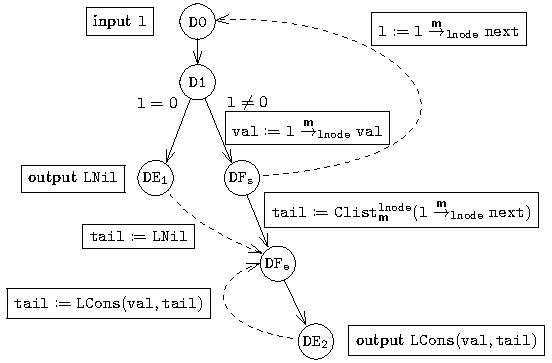
\includegraphics[scale=0.8]{chapters/figures/figClistCfg.pdf}
\vspace{3px}
\caption{\label{fig:reconsProg}Reconstruction Program}
\end{subfigure}%
&
\begin{subfigure}[b]{0.51\textwidth}
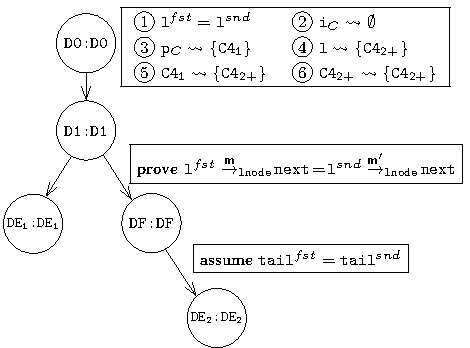
\includegraphics[scale=0.85]{chapters/figures/figClistProductCfg.pdf}
\vspace{17px}
\caption{\label{fig:reconsPCFG}Recons-PCFG}
\end{subfigure}%
%&
%\begin{subfigure}[b]{0.17\textwidth}
%\includegraphics[scale=0.8]{figMallocPointsToGraph.pdf}
%\caption{\label{xxx}XXX}
%\end{subfigure}%
\\
\end{tabular}
\caption{\label{fig:recons}Reconstruction program for \lifted{list}{\mem{}}{lnode}{l} and recons-PCFG between reconstruction programs of \lifted{list}{\mem{}}{lnode}{\cv{l}} and \lifted{list}{\mem{}'}{lnode}{\cv{l}} respectively. \\
In \cref{fig:reconsProg}, the square boxes show the transfer functions based on \cref{eqn:clist}.\\
The dashed edges represent a function call. In \cref{fig:reconsPCFG}, the square box to the \\ right of node (\rrpc{0}{0}) contains the inferred invariants for this recons-PCFG.}
\end{figure}


To check if $\lifted{list}{\mem{}}{lnode}{\cv{l}} \indEq{} \lifted{list}{\mem{}'}{lnode}{\cv{l}}$, we instead
check if a bisimulation relation exists
between the two respective deconstruction programs (assuming \lhs{} as the precondition at entries).
Similar to the top-level bisimulation search, we use a product-CFG to represent this bisimulation relation.
To distinguish this product-CFG from the top-level product-CFG that relates $S$ and $C$, we call
this product-CFG that relates two deconstruction programs, a {\em deconstruction product-CFG}
or {\em decons-PCFG} for short.
% To check bisimulation, we attempt to show that both reconstructions
% proceed in lockstep, and the invariants at
% each step of this lockstep execution ensure equal observables.
% We use a product-CFG to encode this lockstep execution --- to distinguish this
% product-CFG from the top-level product-CFG that relates $S$ and $C$, we call
% this product-CFG that relates two reconstruction programs, a {\em reconstruction product-CFG}
% or {\em decons-PCFG} for short.
% i.e., (1) the first deconstruction procedure evaluates
%an \underline{if} condition (e.g., {\tt l$_C$=0}) to true iff the second
%deconstruction procedure also evaluates the
%corresponding \underline{if} condition to true; and (2)
%the values observed by the first deconstruction procedure (e.g., {\tt lnode.value}
%which is used for constructing the observable {\tt List}) are identical to the
%ones observed by the second deconstruction procedure.
%As we have seen earlier, this lockstep execution can be encoded
%as a product-CFG: the invariants at the nodes of this product-CFG
%represent the conditions that must hold at the correlated
%PCs of this
%lockstep execution; for
%a successful bisimulation check, these invariants must ensure equal observables.
The deconstruction
program and the decons-PCFG for our \lift{list}{\mem{}}{lnode} example are shown in \cref{fig:recons}.
We distinguish states between the first and second programs using superscripts: $fst$ and $snd$ respectively.
However, these are omitted in case the states are equal in both programs (e.g., \cv{p}).
Since both \lifted{list}{\mem{}}{lnode}{\cv{l}}
and \lifted{list}{\mem{}'}{lnode}{\cv{l}} use the same
lifting constructor \lift{list}{\mem{}}{lnode}, the PC-transition correlations of both programs
are trivially obtained by unifying the program structures.
A node is created in the decons-PCFG that
encodes the correlation of the entries to both programs,
we call this node the {\em recursive-node} in the decons-PCFG (e.g., \ddpc{0}{0} in \cref{fig:reconsPCFG}).
A recursive call becomes a back-edge in the decons-PCFG that terminates at the recursive-node.
% A candidate invariant at the recursive-node is obtained by equating the pair of corresponding $l$
% variables across the first (superscripted with $fst$) and second (superscripted with $snd$) programs.
At the start of both deconstruction programs, $\fstv{l} = \sndv{l} = \cv{l}$ --- the same \cv{l} is passed to
both deconstruction programs, only the memory states \mem{} and $\mem{}'$ are different.
The bisimulation check thus involves checking that if the invariant $\fstv{l} = \sndv{l}$
holds at the recursive-node, then during one iteration of the static programs:
\vspace{-13px}
\begin{enumerate}
\setlength{\itemsep}{-3px}
\item The \underline{\tt if} condition $(\fstv{l} = 0)$ in the first program is equal to the corresponding
\underline{\tt if} condition $(\sndv{l} = 0)$ in the second program.
\item If the \underline{\tt if} condition evaluates to false in both programs, then
the observable values (that are used in the construction of the list) are equal: \\
$((\fstv{l} \neq 0) \land (\sndv{l} \neq 0)) \Rightarrow (\structPointer{\fstv{l}}{\mem{}}{lnode}{val} = \structPointer{\sndv{l}}{\mem{}'}{lnode}{val})$.
\item If the \underline{\tt if} condition evaluates to false in both programs, then
the invariant holds at the beginning of the programs invoked through the
recursive call. This involves checking equality of the arguments to the recursive call: \\
$((\fstv{l} \neq 0) \land (\sndv{l} \neq 0)) \Rightarrow (\structPointer{\fstv{l}}{\mem{}}{lnode}{next} = \structPointer{\sndv{l}}{\mem{}'}{lnode}{next})$.
\end{enumerate}
\vspace{-10px}
The first check succeeds due to the invariant $\fstv{l} = \sndv{l}$.
For the second and third checks, we additionally
need to reason that the memory objects
$\structPointer{\comv{l}}{\mem{}}{lnode}{val}$ and $\structPointer{\comv{l}}{\mem{}}{lnode}{next}$ cannot
alias with the writes (in $\mem{}'$ in \cref{eqn:memstore}) to the newly allocated objects
$\structPointer{\cv{p}}{\mem{}}{lnode}{val}$ and $\structPointer{\cv{p}}{\mem{}}{lnode}{next}$.
We capture this aliasing information by running an interprocedural allocation-site based points-to analysis on
the original $C$ program as well as the deconstruction programs being checked
for equivalence. Our points-to analysis also splits each allocation site region, say \mlr{C4} in \cref{fig:llAllocCIR}, into
two regions \mlrf{C4} and \mlrs{C4}, where \mlrf{C4} represents the region of the most recent allocation and \mlrs{C4}
represents the region of all other allocations through ${\tt malloc_{C4}}$ respectively.
We write $p \pointsTo{} \{\mlr{R_1}, \mlr{R_2}\}$ to represent the condition that value $p$ {\em may point to}
an object belonging to one of the region labels \mlr{R_1} or \mlr{R_2}
(but may not point to any object outside of \mlr{R_1} and \mlr{R_2}). We compute may-point-to information for
all program variables as well as the region labels themselves.
% For example, at the start of PC {\tt C7} in \cref{fig:llAllocCIR},
% {\tt i}$_C\pointsTo{}\emptyset$,
% {\tt n}$_C\pointsTo{}\{{\tt C4}_1\}$,
% and {\tt l}$_C\pointsTo{}\{{\tt C4}_{2+}\}$.
% Because the may-point-to analysis determines the
% sets of objects pointed-to by {\tt n}$_C$ and {\tt l}$_C$ to
% be disjoint ($\{{\tt C4_{1}}\}$ vs. $\{{\tt C4_{2+}}\}$), any
% memory accesses through {\tt n}$_C$ and {\tt l}$_C$
% cannot alias at {\tt C7} (for an access
% offset that is within the bounds of
% the allocation size `{\tt sizeof lnode}').
% Similarly, at PC {\tt C7}, we
% get
% ${\tt C4}_{1}\pointsTo{}\{{\tt C4}_{2+}\}$ and
% ${\tt C4}_{2+}\pointsTo{}\{{\tt C4}_{2+}\}$.
% The condition
% ${\tt C4}_{1}\pointsTo{}\{{\tt C4}_{2+}\}$
% holds because the {\tt next} pointer of the object
% pointed-to by ${\tt n}_C$ (which
% is a ${\tt C4}_1$ object) may point to
% a {\tt C4}$_{2+}$ object (e.g., object pointed-to
% by {\tt l}$_C$).
% Similarly, ${\tt C4}_{2+}\pointsTo{}\{{\tt C4}_{2+}\}$
% says that a pointer within a {\tt C4}$_{2+}$ object
% may point to a {\tt C4}$_{2+}$
% object (but not to a {\tt C4}$_1$ object).

% \subsubsection{Transferring points-to information to the decons-PCFG}
% \label{sec:pointsToAsInvariants}
% Recall that
% in \cref{sec:recursiveEqToBisim},
% we reduce a validity check of the condition
% ${\tt Clist}_m^{{\tt lnode}}({\tt l}_C)
% \indEq{} {\tt Clist}_{m'}^{{\tt lnode}}({\tt l}_C)$
% to a bisimulation check. Also, recall
% that we discharge the bisimulation check through the construction
% of a decons-PCFG that compares the unrolling procedure with itself (executing
% on memory states $m$ and $m'$).
% During this bisimulation check, we need to prove
% that for each execution
% of the unrolling procedure, $\structPointer{{\tt l}_C}{m}{\tt lnode}{\{val,next\}}$
% and $\structPointer{{\tt l}_C}{m'}{\tt lnode}{\{val,next\}}$\footnote{Here, we use the symbol {\tt l}$_C$ to
% refer to equal values {\tt l}$^{fst}_C$ and
% {\tt l}$^{snd}_C$.} are equal.
% To successfully discharge these proof obligations, it suffices
% to show ${\tt l}_C$ cannot alias with the memory writes that
% distinguish $m$ from $m'$.
\vspace{-5px}
Our points-to analysis on
the C program determines that at PC \cpc{5} of \cref{fig:llAllocCIR} (the start of
the product-CFG edge \scedge{3}{5}{3}{3} across which the proof
condition is being evaluated), the pointer to the {\em head}
of the list, i.e., $\cv{l} \pointsTo{} \{ \mlrs{C4} \}$.
It also determines that the distinguishing
writes modify memory regions belonging to \mlrf{C4} only.
Further, we get $\mlrs{C4} \pointsTo{} \{ \mlrs{C4} \}$ at PC \cpc{5}.
However, notice that these determinations only rule out aliasing of the list-head with
the distinguishing writes. We also need to confirm non-aliasing
of the internal nodes of the linked list with the distinguishing writes.
For this, we need to identify a points-to invariant,
$\sndv{l} \pointsTo{} \{ \mlrs{C4} \}$, at the recursive-node
of the decons-PCFG (shown in \cref{fig:reconsPCFG}).
To identify such points-to invariant, we run our points-to analysis
on the deconstruction programs (\cref{fig:reconsProg}) before comparing them for equivalence.
To model procedure calls, a {\em supergraph} is created with control flow to and from the entry and exit
of the program (e.g., dashed edges in \cref{fig:recons}).
We use the results of the points-to analysis on $C$ at the PC where the proof obligation
is being discharged (\cpc{5} of \cref{fig:llAllocC} in our case).
To see why $\sndv{l} \pointsTo{} \{ \mlrs{C4} \}$ is
an inductive invariant at the recursive-node:
(base case) the invariant holds at entry to the decons-PCFG since it holds for \cv{l} and
(induction step) if $\sndv{l} \pointsTo{} \{ \mlrs{C4} \}$ holds at the entry node,
it also holds at the start of a recursive call.
This follows from $\mlrs{C4} \pointsTo{} \{ \mlrs{C4} \}$ (points-to information at PC \cpc{5}),
which ensures that $\structPointer{\cv{l}}{\mem{}'}{lnode}{next}$ may point to only \mlrs{C4} objects.
% \vspace{-10px}
% \begin{itemize}
% \setlength{\itemsep}{0px}  
% \item (Base case) The invariant holds
% at entry to the decons-PCFG (because it holds for ${\tt l}^{start}_C$).
% \item (Induction step) If ${\tt l}_C^{snd}\pointsTo{}\{{\tt C4}_{2+}\}$
% holds at the entry node,
% it also holds at the start of a recursive call. This
% follows from ${\tt C4}_{2+}\pointsTo{}\{{\tt C4}_{2+}\}$ (points-to information at PC {\tt C5}),
% which ensures that $\structPointer{\tt l_C}{m'}{\tt lnode}{next}$ may point to only ${\tt C4}_{2+}$ objects.
% \end{itemize}
% \vspace{-10px}
During proof obligation discharge (e.g., during the bisimulation check on decons-PCFG),
the points-to invariants are encoded as SMT constraints.
This allows us to successfully complete the bisimulation proof on the decons-PCFG, and
consequently successfully discharge the proof obligation
\hoareTriple{\scpcinv{3}{5}} {\spath{3,5,3}, \cpath{5,3}}{\sv{l} \indEq{} \lifted{list}{\mem{}}{lnode}{\cv{l}}}
generated due to \circled{\small I4} invariant in \cref{tab:llproductInv}.
% The points-to analysis is described more formally
% in \cref{sec:pointsToFormal}.
\vspace{-10px}
\subsection{Summary of Proof Discharge Algorithm}
\vspace{-5px}
\label{sec:syn-algosummary}
Let $Solve(\lhs{}, \rhs{}, k, d_o, d_u)$ be the top-level procedure for discharging proof obligations.
$\lhs{} \Rightarrow \rhs{}$ represents the proof obligation, where $k$, $d_o$ and $d_u$ are the categorization parameter,
over- and under-approximation depths respectively.
$Solve$ returns either {\tt T} or {\tt F}($\Gamma$) signifying proven and disproven respectively
where $\Gamma$ is a set of counterexamples.
We perform \rhs{}-breaking on the lowered proof obligations and invoke $Solve$ for each smaller proof obligations.
\Cref{algo:proofSummary} gives a broad overview of our proof discharge algorithm.

\begin{figure}[H]
\begin{algorithm}[H]
\begin{scriptsize}
\SetAlgoLined
\SetKwProg{Fn}{Function}{}{end}
\Fn{$Solve(\lhs{}, \rhs{}, k, d_o, d_u)$}{
  $(\lhs{}_k, \rhs{}_k) \mapsfrom DecomposeAndUnroll(\lhs{}, \rhs{}, k)$;\\
  \Switch{$Categorize(\lhs{}_k, \rhs{}_k)$}{
    \lCase{${\tt Type\ I}$}{\Return{$SMTSolve(\lhs{}_k \Rightarrow \rhs{}_k)$}}
    \uCase{${\tt Type\ II}$}{
      $(\lhs{}_o, \lhs{}_u) \mapsfrom Approximate(\lhs{}, d_o, d_u)$;\\
      \lIf{$SMTSolve(\lhs{}_o \Rightarrow \rhs{}_k) \equiv {\tt T}$}{\Return{${\tt T}$}}
      \lIf{$SMTSolve(\lhs{}_u \Rightarrow \rhs{}_k) \equiv {\tt F}(\Gamma)$}{\Return{${\tt F}(\Gamma)$}}
      \lElse{\Return{${\tt F}(\emptyset)$}}
    }
    \Case{${\tt Type\ III}$}{
      \ForEach{${\tt P}_i \Rightarrow \rhs{}_i : DecomposeAndRHSBreak(\lhs{}, \rhs{})$}{
        \uIf{$\rhs{}_i\ \equiv\ l_1\indEq{}l_2$}{
          $(D_1,D_2) \mapsfrom GetDeconstructionPrograms(l_1,l_2)$;\\
          \lIf{$CheckBisimilarity(\lhs{} \land {\tt P}_i,D_1,D_2) \equiv {\tt F}$}{\Return{${\tt F}(\emptyset)$}}
        }
        \Else{
          \lIf{$Solve(\lhs{} \land {\tt P}_i, \rhs{}_i, k, d_o, d_u) \equiv {\tt F}(\Gamma)$}{\Return{${\tt F}(\Gamma)$}}
        }
      }
      \Return{${\tt T}$};
    }
  }
}
\end{scriptsize}
\end{algorithm}
\caption{\label{algo:proofSummary} Summary of the Proof Discharge Algorithm}
\end{figure}

%Thus, as a part of the invariant inference procedure on the product-CFG
%for the decomposition programs, we also run our points-to analysis on the
%product-CFG to identify points-to invariants at the product-CFG
%nodes.  This improves precision, as shown in the example discussed
%above.
% \vspace{-5px}
% \subsubsection{Proof discharge algorithm for Type III obligations}
% \label{sec:cat3summary}

% Before the start of an equivalence check, a points-to analysis is run on the $C$ IR once.
% During the equivalence check,
% to discharge a Type III proof obligation $P: {\tt LHS}\Rightarrow{\tt RHS}$ (expressed
% in first-order logic), we first replace the recursive
% values of program $S$ in the {\tt RHS}
% with lifted C values, based on the equalities present in the {\tt LHS}, to
% obtain $P_2$.
% This is followed by decomposition and RHS-breaking of $P_2$.

% Upon successful decomposition, we
% obtain several smaller proof obligations.
% To prove $P$, we require all these smaller proof
% obligations to be provable. If any of these smaller proof obligations
% is not provable, we are unable to prove $P$.  If we obtain a counterexample
% to any of these smaller proof obligations, then that counterexample
% also falsifies $P$.
% Let $P_3$ represent any such smaller proof obligation.
% {\tt RHS} of $P_3$, being
% a decomposition clause,
% must relate atomic expressions on the {\tt RHS}.
% If $P_3$ relates two scalar values in the {\tt RHS}, then
% it is a Type II proof obligation and can be discharged
% using the algorithm in \cref{sec:cat2algo}.

% If $P_3$ relates two lifted
% expressions in
% the {\tt RHS},
% we check if the reconstruction
% programs of the two lifted ADT values being
% compared can be proven to be bisimilar (assuming that
% {\tt LHS} of $P_3$ holds at the correlated entry nodes
% in the decons-PCFG).
% To improve
% the bisimulation
% check's precision, we transfer the points-to information of the $C$ program
% (at the PC where the proof obligation is being discharged) to the entry
% of the reconstruction programs. The same points-to analysis is ran on the
% reconstruction programs to populate the points-to function at all PCs.

% These queries
% generated by a bisimulation check are discharged
% by a recursive call to the proof discharge procedure.
% The depth of these recursive calls to the
% proof discharge procedure is determined by
% the maximum {\em recursion nest depth} (similar
% to loop nest depth) of the decomposition
% program.

% If the bisimilarity check succeeds, the proof procedure returns
% true for $P$.
% If the bisimilarity check fails,
% we imprecisely return false for $P$ (without a counterexample).

% Finally, if $P_3$ neither
% relates two scalar values, nor relates two lifted expressions,
% we attempt to prove that {\tt LHS} of $P_3$ imply {\tt false}.
% If successfully disproven, we return false for $P$ with the counterexamples.
% Otherwise, we imprecisely return false for $P$ (without a counterexample).

% Please refer to {\tt Chapter \ThesisChapterAlgo{}} of the thesis for a
% detailed discussion on the algorithms introduced in this section along
% with their pseudo-code.
\begin{table}[t]
\caption{\label{tab:LiftingConsStr}String lifting constructors and their definitions.}
\vspace{-5px}
\begin{scriptsize}
\begin{center}
\begin{tabular}{|l|l|}
\hline
\multicolumn{1}{|c|}{\Tstrut \Bstrut\footnotesize Lifting Constructor} & \multicolumn{1}{c|}{\Tstrut \Bstrut \footnotesize Definition} \\
\hline
\hline
% \multicolumn{2}{|c|}{\Tstrut \Bstrut \inv{T1} {\tt List = LNil | LCons(i32, List)}} \\
% \hline
% $\mathrm{Clist^{u32[]}_m(p\ i\ n : i32)}$ & \makecell[l]{\Tstrut $\mathrm{\underline{if}\ (i\geq_{u}n)}$ $\mathrm{\underline{then}\ LNil}$ \\ \Bstrut $\mathrm{\underline{else}\ LCons(p[i]^m_{i32}, Clist^{u32[]}_m(p,i+1_{i32},n))}$} \\
% \hline
% $\mathrm{Clist^{lnode(u32)}_m(p:i32)}$ & \makecell[l]{\Tstrut $\mathrm{\underline{if}\ (p==0_{i32})}$ $\mathrm{\underline{then}\ LNil}$ \\ \Bstrut $\mathrm{\underline{else}\ LCons(\structPointer{\tt p}{m}{\tt lnode}{val}, Clist^{lnode}_m(\structPointer{\tt p}{m}{\tt lnode}{next})}$} \\
% \hline
% $\mathrm{Clist^{clnode(u32)}_m(p:i32,i:i2)}$ & \makecell[l]{\Tstrut $\mathrm{\underline{if}\ (p==0_{i32})}$ $\mathrm{\underline{then}\ LNil}$ \\ \Bstrut $\mathrm{\underline{else}\ LCons(\structPointer{\tt p}{m}{\tt clnode}{chunk}[i]^m_{i32}, Clist^{clnode}_m((ite(i==3_{i2}, \structPointer{\tt p}{m}{\tt clnode}{next},p), i+1_{i2}))}$} \\
% \hline
% $\mathrm{Clist^{u32[r]}_m(p\ i\ j\ u\ v:i32)}$ & \makecell[l]{\Tstrut $\mathrm{\underline{if}\ (j\geq_{u}v)}$ $\mathrm{\underline{then}\ LNil}$ \\ \Bstrut $\mathrm{\underline{else}\ LCons(p[i*v+j]^m_{i32}, Clist^{u32[r]}_m(p,i,j+1_{i32},u,v))}$} \\
% \hline
% $\mathrm{Clist^{u32[c]}_m(p\ i\ j\ u\ v:i32)}$ & \makecell[l]{\Tstrut $\mathrm{\underline{if}\ (j\geq_{u}v)}$ $\mathrm{\underline{then}\ LNil}$ \\ \Bstrut $\mathrm{\underline{else}\ LCons(p[i+j*u]^m_{i32}, Clist^{u32[c]}_m(p,i,j+1_{i32},u,v))}$} \\
% \hline
% \hline
% \multicolumn{2}{|c|}{\Tstrut \Bstrut \inv{T2} {\tt Tree = TNil | TCons(i32, Tree, Tree)}} \\
% \hline
% $\mathrm{Ctree^{u32[]}_m(p\ i\ n : i32)}$ & \makecell[l]{\Tstrut $\mathrm{\underline{if}\ (i \geq_{u} n)}$ $\mathrm{\underline{then}\ TNil}$ \\ \Bstrut $\mathrm{\underline{else}\ TCons(p[i]^{i32}_m, Ctree^{u32[]}_m(p,2_{i32}*i+1_{i32},n), Ctree^{u32[]}_m(p,2_{i32}*i+2_{i32},n))}$ } \\
% \hline
% $\mathrm{Ctree^{tnode(u32)}_m(p:i32)}$ & \makecell[l]{\Tstrut $\mathrm{\underline{if}\ (p==0_{i32})}$ $\mathrm{\underline{then}\ TNil}$ \\ \Bstrut $\mathrm{\underline{else}\ TCons(\structPointer{\tt p}{m}{\tt tnode}{val}, Ctree^{tnode}_m(\structPointer{\tt p}{m}{\tt tnode}{left}), Ctree^{tnode}_m(\structPointer{\tt p}{m}{\tt tnode}{right}))}$ } \\
% \hline
% \hline
\multicolumn{2}{|c|}{\Tstrut \Bstrut \inv{T1} {\tt Str = SInvalid | SNil | SCons(i8, Str)}} \\
\hline
$\mathrm{Cstr^{u8[]}_m(p:i32)}$ & \makecell[l]{\Tstrut $\mathrm{\underline{if}\ (p==0_{i32})}$ $\mathrm{\underline{then}\ SInvalid}$ \\ \Tstrut $\mathrm{\underline{else\ if}\ (p[0_{i32}]^m_{i8}==0_{i8})\ \underline{then}\ SNil}$ \\ \Bstrut $\mathrm{\underline{else}\ SCons(p[0_{i32}]^m_{i8}, Cstr^{u8[]}_m(p+1_{i32}))}$} \\
\hline
$\mathrm{Cstr^{lnode(u8)}_m(p:i32)}$ & \makecell[l]{\Tstrut $\mathrm{\underline{if}\ (p==0_{i32})}$ $\mathrm{\underline{then}\ SInvalid}$ \\ \Tstrut $\mathrm{\underline{else\ if}\ (\structPointer{\tt p}{m}{\tt lnode}{val} == 0_{i8})\ \underline{then}\ SNil}$ \\ \Bstrut $\mathrm{\underline{else}\ SCons(\structPointer{\tt p}{m}{\tt lnode}{val}, Cstr^{lnode(u8)}_m(\structPointer{\tt p}{m}{\tt lnode}{next}))}$} \\
\hline
$\mathrm{Cstr^{clnode(u8)}_m(p:i32,i:i2)}$ & \makecell[l]{\Tstrut $\mathrm{\underline{if}\ (p==0_{i32})}$ $\mathrm{\underline{then}\ SInvalid}$ \\ \Tstrut $\mathrm{\underline{else\ if}\ (\structPointer{\tt p}{m}{\tt clnode}{chunk} [i]^m_{i8} == 0_{i8})\ \underline{then}\ SNil}$ \\ \Bstrut $\mathrm{\underline{else}\ SCons(\structPointer{\tt p}{m}{\tt clnode}{chunk} [i]^m_{i8},}$ \\ \qquad \qquad \quad $\mathrm{Cstr^{clnode(u8)}_m((i==3_{i2}\ ?\ \structPointer{\tt p}{m}{\tt clnode}{next}\ :\ p), i+1_{i2}))}$} \\
\hline
% \hline
% \multicolumn{2}{|c|}{\Tstrut \Bstrut \inv{T4} {\tt Matrix = MNil | MCons(List, Matrix)}} \\
% \hline
% $\mathrm{Cmat^{u32[][]}_m(p\ i\ u\ v:i32)}$ & \makecell[l]{\Tstrut $\mathrm{\underline{if}\ (i \geq_{u} u)}$ $\mathrm{\underline{then}\ MNil}$ \\ \Bstrut $\mathrm{\underline{else}\ MCons(Clist^{u32[]}_m(p[i]^m_{i32},0_{i32},v), Cmat^{u32[][]}_m(p,i+1_{i32},u,v))}$} \\
% \hline
% $\mathrm{Cmat^{u32[r]}_m(p\ i\ u\ v:i32)}$ & \makecell[l]{\Tstrut $\mathrm{\underline{if}\ (i \geq_{u} u)}$ $\mathrm{\underline{then}\ MNil}$ \\ \Bstrut $\mathrm{\underline{else}\ MCons(Clist^{u32[r]}_m(p,i,0_{i32},u,v), Cmat^{u32[r]}_m(p,i+1_{i32},u,v))}$} \\
% \hline
% $\mathrm{Cmat^{u32[c]}_m(p\ i\ u\ v:i32)}$ & \makecell[l]{\Tstrut $\mathrm{\underline{if}\ (i \geq_{u} u)}$ $\mathrm{\underline{then}\ MNil}$ \\ \Bstrut $\mathrm{\underline{else}\ MCons(Clist^{u32[c]}_m(p,i,0_{i32},u,v), Cmat^{u32[c]}_m(p,i+1_{i32},u,v))}$} \\
% \hline
% $\mathrm{Cmat^{lnode(u32[])}_m(p\ v:i32)}$ & \makecell[l]{\Tstrut $\mathrm{\underline{if}\ (p==0_{i32})}$ $\mathrm{\underline{then}\ MNil}$ \\ \Bstrut $\mathrm{\underline{else}\ MCons(Clist^{u32[]}_m(\structPointer{\tt p}{m}{\tt lnode}{val},0_{i32},v),Cmat^{lnode(u32[])}_m(\structPointer{\tt p}{m}{\tt lnode}{next},v))}$} \\
% \hline
% $\mathrm{Cmat^{lnode(u32)[]}_m(p\ i\ u:i32)}$ & \makecell[l]{\Tstrut $\mathrm{\underline{if}\ (i \geq u)}$ $\mathrm{\underline{then}\ MNil}$ \\ \Bstrut $\mathrm{\underline{else}\ MCons(Clist^{lnode(u32)}_m(p[i]^m_{i32}), Cmat^{lnode(u32)[]}_m(p,i+1_{i32},u))}$} \\
% \hline
% $\mathrm{Cmat^{clnode(u32)[]}_m(p\ i\ u:i32)}$ & \makecell[l]{\Tstrut $\mathrm{\underline{if}\ (i \geq u)}$ $\mathrm{\underline{then}\ MNil}$ \\ \Bstrut $\mathrm{\underline{else}\ MCons(Clist^{clnode(u32)}_m(p[i]^m_{i32},0_{i2}), Cmat^{clnode(u32)[]}_m(p,i+1_{i32},u))}$} \\
% \hline
\end{tabular}
\end{center}
\end{scriptsize}
\end{table}
\vspace{-10px}
\section{Evaluation}
\label{sec:syn-eval}
\vspace{-5px}
We have implemented \toolName{} on top of the
Counter tool \cite{oopsla20}.
We use {\em four} SMT solvers running in parallel for solving
SMT proof obligations discharged by our proof discharge algorithm:
{\tt z3-4.8.7}, {\tt z3-4.8.14} \cite{z3},
{\tt Yices2-45e38fc} \cite{yices},
and {\tt cvc4-1.7} \cite{cvc4solver}.
An unroll factor of {\em four} is used to handle loop unrolling in the C implementation.
We use a default value of {\em eight} for
over- and under-approximation depths ($d_o$ and $d_u$).
The default value of
our unrolling parameter $k$ (used for categorization of proof obligations) is {\em five}.

\toolName{} requires the user to provide a \SpecL{} program (specification), a C implementation,
and a file that contains the precondition and postcondition. All inductive invariants
at intermediate nodes in the product-CFG are inferred automatically.
We consider programs involving four distinct ADTs, namely,
\inv{\small T1} \type{String}, \inv{\small T2} \type{List}, \inv{\small T3} \type{Tree}
and \inv{\small T4} \type{Matrix}.

\subsection{Experiments}
For each \SpecL{} program specification, we consider multiple
C implementations that differ in their (a) layout and representation of ADTs, and
(b) algorithmic strategies. For example, a \type{Matrix}, in C, may be laid out
in a two-dimensional array, a one-dimensional array using row or column major
layouts etc. On the other hand, an optimized implementation may choose manual vectorization
of an inner-most loop. Next, we consider each ADT in more detail. For each,
we discuss (a) its corresponding programs, (b) C memory layouts and their lifting
constructors, and (c) varying algorithmic strategies.

\begin{figure}
\begin{subfigure}[b]{0.5\textwidth}
\begin{center}
\begin{allLangEnvFoot}
~{\tiny \textcolor{mygray}{S0:}}~ i32 strlen (Str s) {
~{\tiny \textcolor{mygray}{S1:}}~   i32 len $\coloneqq$ ${\tt 0_{i32}}$;
~{\tiny \textcolor{mygray}{S2:}}~   while $\neg$(s is SNil):
~{\tiny \textcolor{mygray}{S3:}}~     assume $\neg$(s is SInvalid);
~{\tiny \textcolor{mygray}{S4:}}~     // (s is SCons)
~{\tiny \textcolor{mygray}{S5:}}~     s   $\coloneqq$ s.tail;
~{\tiny \textcolor{mygray}{S6:}}~     len $\coloneqq$ len + ${\tt 1_{i32}}$;
~{\tiny \textcolor{mygray}{S7:}}~   return len;
~{\tiny \textcolor{mygray}{SE:}}~ }
\end{allLangEnvFoot}
\end{center}
\caption{\label{fig:llStrlenSpecIR}Strlen specification}
\end{subfigure}%
\begin{subfigure}[b]{0.5\textwidth}
\begin{center}
\vspace{5px}
\begin{allLangEnvFoot}
~{\tiny \textcolor{mygray}{\ \ \ }}~ size_t strlen(char* s);

~{\tiny \textcolor{mygray}{C0:}}~ i32 strlen (i32 s) {
~{\tiny \textcolor{mygray}{C1:}}~   i32 i $\coloneqq$ ${\tt 0_{i32}}$;
~{\tiny \textcolor{mygray}{C2:}}~   while $\arrIndex{\tt s}{0_{i32}}{\mem{}}{i8} \neq 0_{i8}$:
~{\tiny \textcolor{mygray}{C3:}}~     s $\coloneqq$ s + ${\tt 1_{i32}}$;
~{\tiny \textcolor{mygray}{C4:}}~     i $\coloneqq$ i + ${\tt 1_{i32}}$;
~{\tiny \textcolor{mygray}{C5:}}~   return i;
~{\tiny \textcolor{mygray}{CE:}}~ }
\end{allLangEnvFoot}
\end{center}
\caption{\label{fig:llStrlenCArrIR}Generic strlen implementation using array}
\end{subfigure}
\begin{subfigure}[b]{1\textwidth}
\begin{center}
\begin{allLangEnvFoot}
~{\tiny \textcolor{mygray}{\ \ \ \ }}~ typedef struct clnode {
~{\tiny \textcolor{mygray}{\ \ \ \ }}~   char chunk[4]; struct clnode* next; } clnode;
~{\tiny \textcolor{mygray}{\ \ \ \ }}~ size_t strlen(clnode* cl);

~{\tiny \textcolor{mygray}{C0:\phantom{ }}}~ i32 strlen (i32 cl) {
~{\tiny \textcolor{mygray}{C1:\phantom{ }}}~   i32 hi $\coloneqq$ ${\tt 0x80808080_{i32}}$; i32 lo $\coloneqq$ ${\tt 0x01010101_{i32}}$;
~{\tiny \textcolor{mygray}{C2:\phantom{ }}}~   i32 i  $\coloneqq$ ${\tt 0_{i32}}$;
~{\tiny \textcolor{mygray}{C3:\phantom{ }}}~   while ${\tt true}$:
~{\tiny \textcolor{mygray}{C4:\phantom{ }}}~     i32 dword_ptr $\coloneqq$ addrof($\structPointer{\tt cl}{\mem{}}{clnode}{chunk}$);
~{\tiny \textcolor{mygray}{C5:\phantom{ }}}~     i32 dword     $\coloneqq$ $\arrIndex{\tt dword\_ptr}{0_{i32}}{\mem{}}{i32}$;
~{\tiny \textcolor{mygray}{C6:\phantom{ }}}~     if ${\tt ((dword - lo)\ \&\ (\sim dword)\ \&\ hi) \neq 0_{i32}}$:
~{\tiny \textcolor{mygray}{C7:\phantom{ }}}~       if $\arrIndex{\tt dword\_ptr}{0_{i32}}{\mem{}}{i8} = 0_{i8}$: return i;
~{\tiny \textcolor{mygray}{C8:\phantom{ }}}~       if $\arrIndex{\tt dword\_ptr}{1_{i32}}{\mem{}}{i8} = 0_{i8}$: return ${\tt i + 1_{i32}}$;
~{\tiny \textcolor{mygray}{C9:\phantom{ }}}~       if $\arrIndex{\tt dword\_ptr}{2_{i32}}{\mem{}}{i8} = 0_{i8}$: return ${\tt i + 2_{i32}}$;
~{\tiny \textcolor{mygray}{C10:}}~       if $\arrIndex{\tt dword\_ptr}{3_{i32}}{\mem{}}{i8} = 0_{i8}$: return ${\tt i + 3_{i32}}$;
~{\tiny \textcolor{mygray}{C11:}}~     cl $\coloneqq$ $\structPointer{\tt cl}{\mem{}}{clnode}{next}$; i  $\coloneqq$ ${\tt i + 4_{i32}}$;
~{\tiny \textcolor{mygray}{CE:\phantom{ }}}~ }
\end{allLangEnvFoot}
\end{center}
\caption{\label{fig:llStrlenCClistIR}Optimized strlen implementation using chunked linked list}
\end{subfigure}%
\caption{\label{fig:strlenSpecAndC}\Cref{fig:llStrlenSpecIR} shows the (abstracted) IR for the \SpecL{} specification of {\tt strlen}.
\Cref{fig:llStrlenCArrIR,fig:llStrlenCClistIR} show the (abstracted) IRs for two C implementations of {\tt strlen}.
\Cref{fig:llStrlenCArrIR} is a generic implementation using a nul-terminated array to represent a string, whereas
\cref{fig:llStrlenCClistIR} is an optimized implementation with a chunked linked list memory layout for a string.}
\end{figure}


\subsubsection{String}
We wrote a single specification in \SpecL{} for each of the
following common string library functions: {\tt strlen}, {\tt strchr}, {\tt strcmp}, {\tt strspn},
{\tt strcspn}, and {\tt strpbrk}.  For each specification
program, we took multiple C implementations of that program, drawn from popular
libraries like {\tt glibc} \cite{glibc}, {\tt klibc} \cite{klibc}, {\tt newlib} \cite{newlib},
{\tt openbsd} \cite{openbsdlibc}, {\tt uClibc} \cite{uclibc},
{\tt dietlibc} \cite{dietlibc}, {\tt musl} \cite{musl}, and {\tt netbsd} \cite{netbsd}.
Some of these libraries implement the same function in two ways: one that is optimized
for code size and another that is optimized for runtime.
All these library implementations use a {\em null character} terminated array to represent
a string, and the
corresponding lifting constructor is \lift{str}{\mem{}}{u8[]}.
\type{u<N>} represents the N-bit unsigned integer type in C.
For example, \type{u8} represents \type{unsigned char} type.

Further, we implemented
custom C programs for all of these functions that used
linked list
and {\em chunked linked list} data structures
to represent a string.
In a chunked linked list, a single list node (linked
through a {\tt next} pointer)
contains a small array (chunk) of values.
We use a default chunk size of four for our
benchmarks.
The corresponding lifting constructors are \lift{str}{\mem{}}{lnode(u8)}
and \lift{str}{\mem{}}{clnode(u8)} respectively.
These lifting constructors are defined in \cref{tab:LiftingConsStr}.
\lift{str}{\mem{}}{lnode(u8)} requires a single
argument $p$ representing the pointer to the list node.
On the other hand, \lift{str}{\mem{}}{clnode(u8)} requires two arguments $p$
and $i$, where $p$ represents the pointer to the chunked linked list node
and $i$ represents the position of the initial character in the chunk.

\Cref{fig:strlenSpecAndC} shows the {\tt strlen} specification and two vastly
different $C$ implementations. \Cref{fig:llStrlenCArrIR} is a generic implementation
using a null character terminated array to represent a string similar to a C-style string.
The second implementation in \cref{fig:llStrlenCClistIR} differs from \cref{fig:llStrlenCArrIR}
in the following: (a) it uses a chunked linked list data layout for the input string
and (b) it uses specialized bit manipulations to identify a null character in a chunk at a time.
\toolName{} is able to automatically find a bisimulation relation
for both implementations against the unaltered specification.
\Cref{fig:StrlenProductCFGsAndInvs} shows the product-CFG and invariants for each implementation.

\begin{figure}[t!]
\begin{tabular}{@{}c@{}c@{}}
\begin{subfigure}[b]{0.50\textwidth}
\begin{center}
{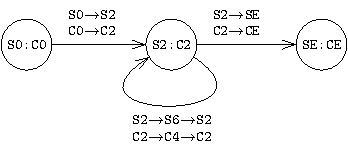
\includegraphics[scale=1.2]{chapters/figures/figStrlenArrProductCfg.pdf}}
\end{center}
\caption{\label{fig:StrlenArrProductCFG}Product-CFG for programs \cref{fig:llStrlenSpecIR,fig:llStrlenCArrIR}}
\end{subfigure}%
&
\begin{subfigure}[b]{0.50\textwidth}
\begin{center}
\begin{scriptsize}
\begin{tabular}{cl}
\toprule
{\bf PC-Pair} & \multicolumn{1}{c} {\bf Invariants} \\
\toprule
(\scpc{0}{0}) &
\Tstrut $\circled{P}\ \sv{s} \indEq{} \lifted{str}{\mem{}}{char[]}{\cv{s}}$ \\
\midrule
\multirow{2}{*}{(\scpc{2}{2})} &
\Tstrut $\circled{\tiny I1} \ \sv{s} \indEq{} \lifted{str}{\mem{}}{char[]}{\cv{s}}$ \\ &
\Tstrut $\circled{\tiny I2} \ \sv{len} = \cv{i}$ \\
\midrule
(\scpc{E}{E}) &
\Tstrut \Bstrut $\circled{E}\ \sv{ret} = \cv{ret}$ \\
\bottomrule
\end{tabular}
\end{scriptsize}
\end{center}
\caption{\label{fig:StrlenArrInvs}Invariants for product-CFG in \cref{fig:StrlenArrProductCFG}}
\end{subfigure}%
\\
\begin{subfigure}[b]{0.50\textwidth}
\begin{center}
{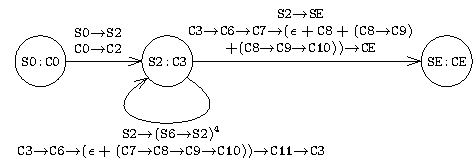
\includegraphics[scale=1.15]{chapters/figures/figStrlenClProductCfg.pdf}}
\end{center}
\caption{\label{fig:StrlenClProductCFG}Product-CFG for programs \cref{fig:llStrlenSpecIR,fig:llStrlenCClistIR}}
\end{subfigure}%
&
\begin{subfigure}[b]{0.50\textwidth}
\begin{center}
\begin{scriptsize}
\begin{tabular}{cl}
\toprule
{\bf PC-Pair} & \multicolumn{1}{c} {\bf Invariants} \\
\toprule
(\scpc{0}{0}) &
\Tstrut $\circled{P}\ \sv{s} \indEq{} \lifted{str}{\mem{}}{clnode}{\cv{cl},0}$ \\
\midrule
\multirow{2}{*}{(\scpc{2}{3})} &
\Tstrut $\circled{\tiny I1} \ \sv{s} \indEq{} \lifted{str}{\mem{}}{clnode}{\cv{cl},0}$ \\ &
\Tstrut $\circled{\tiny I2} \ \sv{len} = \cv{i}$ \\
\midrule
(\scpc{E}{E}) &
\Tstrut \Bstrut $\circled{E} \ \sv{ret} = \cv{ret}$ \\
\bottomrule
\end{tabular}
\end{scriptsize}
\end{center}
\caption{\label{fig:StrlenClInvs}Invariants for product-CFG in \cref{fig:StrlenClProductCFG}}
\end{subfigure}%
\end{tabular}
\caption{\label{fig:StrlenProductCFGsAndInvs}Product-CFGs and their node invariants representing bisimulation relations between the specification \cref{fig:llStrlenSpecIR}
and its two implementations in \cref{fig:llStrlenCArrIR,fig:llStrlenCClistIR} respectively.}
\end{figure}

Lifting constructors are named based on the C data layout being lifted
and the \SpecL{} ADT type of the lifted value.
For example, \lift{str}{}{u8[]} represents a \type{String} lifting constructor
for an array layout.
In general, we use the following naming convention for different C data layouts:
\type{T[]} represents an array of type \type{T} (e.g., \type{u8[]}).
\type{lnode(T)} represents a linked list node type containing a value of type \type{T}.
Similarly, \type{clnode(T)} and \type{tnode(T)} represent a chunked linked list and a tree node
with values of type \type{T} respectively.

\begin{center}
\begin{table}[H]
\begin{scriptsize}
\begin{tabular}{|l|l|}
\hline
\multicolumn{1}{|c|}{\Tstrut \Bstrut\footnotesize Lifting Constructor} & \multicolumn{1}{c|}{\Tstrut \Bstrut \footnotesize Definition} \\
\hline
\hline
\multicolumn{2}{|c|}{\Tstrut \Bstrut \inv{T1} {\tt Str = SInvalid | SNil | SCons(ch:i8, tail:Str)}} \\
\hline
$\mathrm{Cstr^{char[]}_m(p:i32)}$ & \makecell[l]{\Tstrut $\mathrm{\underline{if}\ (p==0_{i32})}$ $\mathrm{\underline{then}\ SInvalid}$ \\ \Tstrut $\mathrm{\underline{else\ if}\ (p[0_{i32}]^m_{i8}==0_{i8})\ \underline{then}\ SNil}$ \\ \Bstrut $\mathrm{\underline{else}\ SCons(p[0_{i32}]^m_{i8}, Cstr^{char[]}_m(p+1_{i32}))}$} \\
\hline
$\mathrm{Cstr^{lnode(char)}_m(p:i32)}$ & \makecell[l]{\Tstrut $\mathrm{\underline{if}\ (p==0_{i32})}$ $\mathrm{\underline{then}\ SInvalid}$ \\ \Tstrut $\mathrm{\underline{else\ if}\ (\structPointer{\tt p}{m}{\tt lnode}{val} == 0_{i8})\ \underline{then}\ SNil}$ \\ \Bstrut $\mathrm{\underline{else}\ SCons(\structPointer{\tt p}{m}{\tt lnode}{val}, Cstr^{lnode}_m(\structPointer{\tt p}{m}{\tt lnode}{next}))}$} \\
\hline
$\mathrm{Cstr^{clnode(char)}_m(p:i32,i:i2)}$ & \makecell[l]{\Tstrut $\mathrm{\underline{if}\ (p==0_{i32})}$ $\mathrm{\underline{then}\ SInvalid}$ \\ \Tstrut $\mathrm{\underline{else\ if}\ (\structPointer{\tt p}{m}{\tt clnode}{chunk} [i]^m_{i8} == 0_{i8})\ \underline{then}\ SNil}$ \\ \Bstrut $\mathrm{\underline{else}\ SCons(\structPointer{\tt p}{m}{\tt clnode}{chunk} [i]^m_{i8},}$ \\ \qquad \qquad \quad $\mathrm{Cstr^{clnode}_m((ite(i==3_{i2},\structPointer{\tt p}{m}{\tt clnode}{next} , p), i+1_{i2}))}$} \\
\hline
\end{tabular}
\end{scriptsize}
\caption{\label{tab:LiftingConsStr}Lifting constructors and their definitions for {\tt String} ADT.}
\vspace{-18px}
\end{table}
\end{center}

\vspace{-15px}
\subsubsection{List}
\vspace{-5px}
We wrote a \SpecL{} program specification that creates a list, a
program that traverses a list to compute the sum of its elements and a program
that computes the dot product of two lists. We use three different
data layouts for a list in C: array (\lift{list}{\mem{}}{u32[]}),
linked list (\lift{list}{\mem{}}{lnode(u32)}), and
a chunked linked list (\lift{list}{\mem{}}{clnode(u32)}).
The lifting constructors are shown in \cref{tab:LiftingConsList}.
Although similar to the String lifting constructors, these lifting
constructors differ widely in their data encoding. For example,
\lifted{list}{\mem{}}{u32[]}{p,i,n} represents a \type{List} value constructed
from a C array $p$ of size $n$ starting at the $i^{th}$ index. The list becomes empty
when we are at the end of the array. (\lift{list}{\mem{}}{lnode(u32)})
and (\lift{list}{\mem{}}{clnode(u32)}), on the other hand, encodes empty
lists (\cons{LNil}) using {\em null pointers}. These layouts are in contrast to the
\type{String} layouts, all of which uses a {\em null character} to
indicate the empty string.

\begin{table}[H]
\begin{center}
\caption{\label{tab:LiftingConsTree}Tree lifting constructors and their definitions.}
\begin{scriptsize}
\begin{tabular}{|l|l|}
\hline
\multicolumn{1}{|c|}{\Tstrut \Bstrut\footnotesize \bf Lifting Constructor} & \multicolumn{1}{c|}{\Tstrut \Bstrut \footnotesize \bf Definition} \\
\hline
\hline
\multicolumn{2}{|c|}{\Tstrut \Bstrut \inv{T3} {\tt Tree = TNil | TCons(i32, Tree, Tree)}} \\
\hline
\lifted{tree}{\mem{}}{u32[]}{p\ i\ n\ctype{i32}} & \makecell[l]{\Tstrut \sumIf{i \geq_u n} \  \sumThen{\cons{TNil}} \\
                                                        \Tstrut \Bstrut \sumElse{\cons{TCons}(\arrIndex{p}{i}{i32}{\mem{}}, \lifted{tree}{\mem{}}{u32[]}{p,2_\type{i32} \times i+1_\type{i32},n}, \lifted{tree}{\mem{}}{u32[]}{p,2_\type{i32} \times i+2_\type{i32},n})}} \\
\hline
\lifted{tree}{\mem{}}{tnode(u32)}{p\ctype{i32}} & \makecell[l]{\Tstrut \sumIf{p = 0_\type{i32}} \  \sumThen{\cons{TNil}} \\
                                                       \Tstrut \Bstrut \sumElse{\cons{TCons}(\structPointer{p\!}{\mem{}}{tnode}{\!\!val},\! \lifted{tree}{\mem{}}{tnode(u32)}{\structPointer{p\!}{\mem{}}{tnode}{\!\!left}},\! \lifted{tree}{\mem{}}{tnode(u32)}{\structPointer{p\!}{\mem{}}{tnode}{\!\!right}})}} \\
\hline
\end{tabular}
\end{scriptsize}
\end{center}
\end{table}
\vspace{-15px}
\subsubsection{Tree}
\vspace{-5px}
We wrote a \SpecL{} program that sums all the nodes in a tree
through an inorder traversal using recursion. We use two different data layouts for a tree: 
(1) a flat array where a
complete binary tree is laid out in breadth-first search order commonly used for heaps (\lift{tree}{\mem{}}{u32[]}),
and (2) a linked tree node with two pointers for the left and right children (\lift{tree}{\mem{}}{tnode(u32)}) (shown in \cref{tab:LiftingConsTree}).
Both \SpecL{} and C programs contain non-tail recursive procedure calls for left and right children.
\toolName{} is able to correlate these recursive calls using user-provided $Pre$ and $Post$.
At the entry of the recursive calls, \toolName{} is required to prove that $Pre$ holds for the arguments
and at the exit of the recursive calls, \toolName{} assumes $Post$ on the returned states.

\begin{table}[H]
\caption{\label{tab:LiftingConsMatrix}Matrix and auxiliary lifting constructors and their definitions.}
\vspace{-10px}
\begin{scriptsize}
\begin{center}
\begin{tabular}{|l|l|}
\hline
\multicolumn{1}{|c|}{\Tstrut \Bstrut\footnotesize Lifting Constructor} & \multicolumn{1}{c|}{\Tstrut \Bstrut \footnotesize Definition} \\
\hline
\hline
\multicolumn{2}{|c|}{\Tstrut \Bstrut \inv{T4} {\tt Matrix = MNil | MCons(List, Matrix)}} \\
\hline
$\mathrm{Cmat^{u32[][]}_m(p\ i\ u\ v:i32)}$ & \makecell[l]{\Tstrut $\mathrm{\underline{if}\ (i \geq_{u} u)}$ $\mathrm{\underline{then}\ MNil}$ \\ \Bstrut $\mathrm{\underline{else}\ MCons(Clist^{u32[]}_m(p[i]^m_{i32},0_{i32},v), Cmat^{u32[][]}_m(p,i+1_{i32},u,v))}$} \\
\hline
\hline
$\mathrm{Clist^{u32[r]}_m(p\ i\ j\ u\ v:i32)}$ & \makecell[l]{\Tstrut $\mathrm{\underline{if}\ (j\geq_{u}v)}$ $\mathrm{\underline{then}\ LNil}$ \\ \Bstrut $\mathrm{\underline{else}\ LCons(p[i*v+j]^m_{i32}, Clist^{u32[r]}_m(p,i,j+1_{i32},u,v))}$} \\
\hline
$\mathrm{Cmat^{u32[r]}_m(p\ i\ u\ v:i32)}$ & \makecell[l]{\Tstrut $\mathrm{\underline{if}\ (i \geq_{u} u)}$ $\mathrm{\underline{then}\ MNil}$ \\ \Bstrut $\mathrm{\underline{else}\ MCons(Clist^{u32[r]}_m(p,i,0_{i32},u,v), Cmat^{u32[r]}_m(p,i+1_{i32},u,v))}$} \\
\hline
\hline
$\mathrm{Clist^{u32[c]}_m(p\ i\ j\ u\ v:i32)}$ & \makecell[l]{\Tstrut $\mathrm{\underline{if}\ (j\geq_{u}v)}$ $\mathrm{\underline{then}\ LNil}$ \\ \Bstrut $\mathrm{\underline{else}\ LCons(p[i+j*u]^m_{i32}, Clist^{u32[c]}_m(p,i,j+1_{i32},u,v))}$} \\
\hline
$\mathrm{Cmat^{u32[c]}_m(p\ i\ u\ v:i32)}$ & \makecell[l]{\Tstrut $\mathrm{\underline{if}\ (i \geq_{u} u)}$ $\mathrm{\underline{then}\ MNil}$ \\ \Bstrut $\mathrm{\underline{else}\ MCons(Clist^{u32[c]}_m(p,i,0_{i32},u,v), Cmat^{u32[c]}_m(p,i+1_{i32},u,v))}$} \\
\hline
\hline
$\mathrm{Cmat^{lnode(u32[])}_m(p\ v:i32)}$ & \makecell[l]{\Tstrut $\mathrm{\underline{if}\ (p==0_{i32})}$ $\mathrm{\underline{then}\ MNil}$ \\ \Bstrut $\mathrm{\underline{else}\ MCons(Clist^{u32[]}_m(\structPointer{\tt p}{m}{\tt lnode}{val},0_{i32},v),}$ \\ \qquad\qquad\ \ \ \  $\mathrm{Cmat^{lnode(u32[])}_m(\structPointer{\tt p}{m}{\tt lnode}{next},v))}$} \\
\hline
$\mathrm{Cmat^{lnode(u32)[]}_m(p\ i\ u:i32)}$ & \makecell[l]{\Tstrut $\mathrm{\underline{if}\ (i \geq u)}$ $\mathrm{\underline{then}\ MNil}$ \\ \Bstrut $\mathrm{\underline{else}\ MCons(Clist^{lnode(u32)}_m(p[i]^m_{i32}),}$ \\ \qquad\qquad\ \ \ \  $\mathrm{Cmat^{lnode(u32)[]}_m(p,i+1_{i32},u))}$} \\
\hline
$\mathrm{Cmat^{clnode(u32)[]}_m(p\ i\ u:i32)}$ & \makecell[l]{\Tstrut $\mathrm{\underline{if}\ (i \geq u)}$ $\mathrm{\underline{then}\ MNil}$ \\ \Bstrut $\mathrm{\underline{else}\ MCons(Clist^{clnode(u32)}_m(p[i]^m_{i32},0_{i2}),}$ \\ \qquad\qquad\ \ \ \  $\mathrm{Cmat^{clnode(u32)[]}_m(p,i+1_{i32},u))}$} \\
\hline
\end{tabular}
\end{center}
\end{scriptsize}
\end{table}

\vspace{-10px}
\subsubsection{Matrix}
We wrote a
\SpecL{} program to count the frequency of a value appearing in a 2D matrix.
A matrix is represented as an ADT that resembles a \type{List} of \type{List}s (\inv{\small T4} in \cref{tab:LiftingConsMatrix}).
The C implementations for a \type{Matrix} object include
(a) a two-dimensional array (\lift{mat}{\mem{}}{u32[][]}), (b) a flattened row-major array (\lift{mat}{\mem{}}{u32[r]}),
(c) a flattened column-major array (\lift{mat}{\mem{}}{u32[c]}), (d) a linked list of 1D arrays (\lift{mat}{\mem{}}{lnode(u32[])}),
(e) a 1D array of linked lists (\lift{mat}{\mem{}}{lnode(u32)[]}) and (f) a 1D array of chunked linked list (\lift{mat}{\mem{}}{clnode(u32)[]})
data layouts. Note that both \type{T[r]} and \type{T[c]} represent a 1D array of type {\tt T}. The {\em r} and {\em c} simply
emphasizes that these arrays are used to represent matrices in row-major and column-major encodings respectively.
We also introduce two auxiliary lifting constructors, \lift{list}{\mem{}}{u32[r]} and \lift{list}{\mem{}}{u32[c]}
for lifting each row of matrices lifted using the corresponding \lift{mat}{\mem{}}{u32[r]} and \lift{mat}{\mem{}}{u32[c]} \type{Matrix} lifting
constructors. These constructors are listed in \cref{tab:LiftingConsMatrix}.
% \vspace{-10px}
\subsection{Results}
\Cref{tab:results} lists the various C implementations and the time it took
to compute equivalence with their specifications. For functions that
take two or more data structures as arguments, we show
results for different combinations of data layouts for {\parfillskip=0pt\par}
\begin{figure}[H]
\begin{scriptsize}
\begin{tabular}{lllclllc}
\toprule
{\bf Data Layout} & {\bf Variant} & {\bf Time(s)} & {\bf ${\tt \bf ( d_u, d_o )}$} & {\bf Data Layout} & {\bf Variant} & {\bf Time(s)} & {\bf ${\tt \bf ( d_u, d_o )}$} \\
\midrule
\multicolumn{4}{c}{\bf list} &                                              \multicolumn{4}{c}{\bf tree} \\
u32[] & sum naive & 16 & (1,2) &                                           u32[] & sum & 264 & (1,2) \\
      & sum opt & 49 & (4,5) &                                             tnode(u32) & sum & 204 & (1,2) \\
lnode(u32) & sum naive & 8 & (1,2) &                                      \multicolumn{4}{c}{\bf matfreq} \\             
           & sum opt & 54 & (4,5) &                                       char[][] & naive & 974 & (1,3) \\                                      
           & create & 426 & (1,1) &                                                & opt & 1.8k & (4,8) \\                                       
clnode(u32) & sum opt & 39 & (4,5) &                                      char[r] & naive & 958 & (1,3) \\                                       
\multicolumn{4}{c}{\bf strlen}   &                                            & opt & 1.9k & (4,8) \\                                        
char[] & dietlibc$\mathrm{_{small}}$ & 9 & (1,2) &                             char[c] & naive & 984 & (1,3) \\                                       
       & dietlibc$\mathrm{_{fast}}$ & 44 & (3,2) &                                     & opt & 1.9k & (4,6) \\
       & glibc & 52 & (3,2) &                                                  lnode(char[]) & naive & 753 & (1,3) \\
       & klibc & 9 & (1,2) &                                                         & opt & 1.7k & (4,6) \\ 
       & musl & 49 & (3,2) &                                                   lnode(char)[] & naive & 1.5k & (1,2) \\
       & netbsd & 9 & (1,2) &                                                                & opt & 2.3k & (4,6) \\
       & newlib & 50 & (3,2) &                                              clnode(char)[] & opt & 1.8k & (4,6) \\
       & openbsd & 8 & (1,2) &                                                \multicolumn{4}{c}{\bf strpbrk} \\ 
       & uClibc & 8 & (1,2) &                                                 char[], char[] & dietlibc & 398 & (1,2) \\
lnode(char) & naive & 13 & (1,2) &                                                          & opt      & 494 & (4,2) \\
            & opt & 49 & (3,5) &                                              char[], lnode(char) & naive & 392 & (1,2) \\
clnode(char) & opt & 45 & (3,5) &                                                                & opt & 540 & (4,2) \\ 
 \multicolumn{4}{c}{\bf strchr} &                                                 char[], clnode(char) & opt & 523 & (4,2) \\
char[] & dietlibc$\mathrm{_{small}}$ & 16 & (1,1) &                           lnode(char), char[] & naive & 497 & (1,2) \\
       & dietlibc$\mathrm{_{fast}}$ & 89 & (4,1) &                                               & opt & 602 & (4,2) \\ 
       & glibc & 127 & (4,1) &                                                lnode(char), lnode(char) & naive & 345 & (1,2) \\
       & klibc & 23 & (1,1) &                                                                           & opt & 503 & (4,2) \\
       & newlib$\mathrm{_{small}}$ & 15 & (1,1) &                         lnode(char), clnode(char) & opt & 572 & (4,2) \\
       & openbsd & 24 & (1,1) &                                             \multicolumn{4}{c}{\bf strcspn} \\
       & uClibc & 22 & (1,1) &                                              char[], char[] & dietlibc & 462 & (1,2) \\ 
lnode(char) & naive & 19 & (1,1) &                                                        & opt      & 538 & (4,2) \\ 
            & opt & 146 & (4,1) &                                           char[], lnode(char) & naive & 395 & (1,2) \\
\multicolumn{4}{c}{\bf strcmp}   &                                     & opt & 521 & (4,2) \\
char[], char[] & dietlibc$\mathrm{_{small}}$ & 39 & (1,1) &                 char[], clnode(char) & opt & 527 & (4,2) \\
       & freebsd & 39 & (1,1) &                                             lnode(char), char[] & naive & 601 & (1,2) \\
       & glibc & 41 & (1,1) &                                                                  & opt & 660 & (4,2) \\ 
       & klibc & 41 & (1,1) &                                               lnode(char), lnode(char) & naive & 349 & (1,2) \\
       & musl & 41 & (1,1) &                                                                        & opt & 502 & (4,2) \\
       & netbsd & 39 & (1,1) &                                              lnode(char), clnode(char) & opt & 595 & (4,2) \\
       & newlib$\mathrm{_{small}}$ & 42 & (1,1) &                              \multicolumn{4}{c}{\bf strspn} \\
       & newlib$\mathrm{_{fast}}$ & 405 & (4,1) &                              char[], char[] & dietlibc & 277 & (1,2)                   \\
       & openbsd & 40 & (1,1) &                                                              & opt      & 388 & (4,2)                    \\
       & uClibc & 38 & (1,1) &                                                 char[], lnode(char) & naive & 405 & (1,2)                 \\
lnode(char), lnode(char) & naive & 47 & (1,1) &                                                   & opt & 682 & (4,2)                    \\ 
            & opt & 293 & (4,1) &                                              char[], clnode(char) & opt & 535 & (4,2)                  \\
clnode(char), clnode(char) & opt & 254 & (4,1) &                               lnode(char), char[] & naive & 409 & (1,2)           \\
\multicolumn{4}{c}{\bf vecdot} &                                                          & opt & 553 & (4,2)              \\
u32[] & naive & 65 & (1,2) &                                                  lnode(char), lnode(char) & naive & 357 & (1,2)        \\
      & opt & 176 & (4,5)   &                                                                          & opt & 514 & (4,2)        \\
lnode(u32) & naive & 37 & (1,2) &                                              lnode(char), clnode(char) & opt & 616 & (4,2)         \\
           & opt & 120 & (4,5)   &                                               & & & \\
clnode(u32) & opt & 118 & (4,5)   &                                               & & & \\
\bottomrule
\end{tabular}
\end{scriptsize}
\vspace{-5px}
\caption{\label{tab:results}Equivalence checking times and minimum under- and over-approximation depth values at which equivalence checks succeeded.}
\vspace{-5px}
\end{figure}
\noindent each argument.
We also show the minimum under-approximation ($d_u$) and over-approximation ($d_o$) depths
at which the equivalence proof completed (keeping all other parameters to their
default values).
% \vspace{15px}

\vspace{-12px}
\section{Limitations}
\vspace{-10px}
\label{sec:syn-limitations}
Our proof discharge algorithm is not without limitations.
For a \recursiveRelation{} relating values of a non-linear ADT such as \type{Tree}, a $d$-depth
approximation results in $\sim 2^d$ smaller equalities. This is a major cause of inefficiency due to
generation of large queries which slows down SMT solvers and counterexample-guided algorithms for large values of $d$.

\toolName{} is only interested in finding a bisimulation relation and hence
equivalence of non-bisimilar programs is beyond our scope.
\toolName{} currently only supports bitvector affine and inequality relations
along with \recursiveRelations{} provided as part of $Pre$ and $Post$.
Consequently, non-linear bitvector invariants (e.g. polynomial invariants)
as well as custom \recursiveRelations{} are not supported.
While our correlation and invariant inference algorithms based on the Counter tool \cite{oopsla20}
are designed for translation validation between (C-like) unoptimized IR and assembly, we found them
to be surprisingly good for \SpecL{} to (C-like) IR as well. Rather unsurprisingly, \toolName{}
suffers from the same limitations of these algorithms. For example, \toolName{} supports path
specializations from \SpecL{} to C, it does not search for path merging correlations.
\vspace{-12px}
\section{Conclusion}
\vspace{-10px}
\label{sec:syn-conclusion}
As introduced in \cref{sec:syn-intro}, most of the current solutions
to the problem of equivalence checking between a functional specification
and a C program relies heavily on manually provided correlation, inductive
invariants as well as proof assistants for discharging said obligations.
While the size of programs considered in our work is quite small,
we hope the ideas in \toolName{} will help
automate the proofs for such systems to some degree.

Prior work on push-button verification of specific
systems \cite{fscq,hyperkernel,serval,verifiedBPF}
involves a combination of careful system design and
automatic verification tools like SMT solvers.
Constrained Horn Clause (CHC) Solvers \cite{CHCeq}
encode verification conditions of programs containing loops and recursion,
and raise the level of abstraction for automatic proofs.
Comparatively, \toolName{} further raises the level
of abstraction for automatic verification from
SMT queries and CHC queries to automatic discharge of
proof obligations involving \recursiveRelations{}.

A key idea in \toolName{} is the conversion of proof
obligations involving \recursiveRelations{} to
bisimulation checks. Thus, \toolName{} performs {\em nested}
bisimulation checks as part of a `higher-level'
bisimulation search. This approach of
identifying \recursiveRelations{} as invariants and using
bisimulation to discharge the associated
proof obligations may have applications
beyond equivalence checking.

\vspace{-12px}
\section{Outline of the Thesis}
\vspace{-10px}
\label{sec:outlinethesis}
\textbf{Chapter 1} of the thesis contains a general introduction to the research problem of verification C programs against a functional specification.
We take a C program and its analogue in a safe functional language, and contrast their differences. This helps us motivate the problem and its solution.
We finish with our contributions.

In \textbf{Chapter 2}, we constrain the programs being considered by formulating the problem statement. This helps us define the scope of our solution.
We introduce a custom minimal functional language called `Spec' and define the necessary terminology used in the rest of the thesis.

\textbf{Chapter 3} starts with background on program equivalence, bisimulation relation and product program.
The rest of the chapter gradually introduces our first contribution: A Proof Discharge Algorithm and related sub-procedures with the help
of two example programs. We also introduce a program representation of values, called `reconstruction program'.

Next, we formalize previously discussed topics in \textbf{Chapter 4}. We begin with the specification of our custom language `Spec'.
We give a detailed description of (a) a counterexample-guided search algorithm for finding a bisimulation relation and (b) a counterexample-guided
invariant inference procedure. There two procedures with our proof discharge algorithm allow automatic end-to-end equivalence checking.
We formalize handling of procedure calls in `Spec' as well as C, and finish with a dataflow analysis formulation of a pointer analysis
used by our equivalence checker.

\textbf{Chapter 5} introduces a program graph representation of values, called `deconstruction procedure', similar to `reconstruction procedure' as introduced in \textbf{Chapter 3}.
We motivate it by listing its advantages and give an algorithm to convert expressions to this representation.
This helps us simplify our proof discharge algorithm.

In \textbf{Chapter 6}, we introduce our automatic equivalence checker tool named \toolName{}, based on our proof discharge algorithm
and counterexample-guided search procedures.
\toolName{} is evaluated on a large variety of C programs involving lists, strings, trees and matrices.
This includes C programs taken from C library implementations as well as manually written programs. We show that our equivalence checker is able
to prove equivalence of a single specification with multiple of C implementations, each varying in its data layouts and algorithmic
strategies.

Finally, \textbf{Chapter 7} discusses the limitations of our algorithm and compares it with some related work. We note our major ideas and finish with
some potential future improvements to our algorithm.
\begin{singlespace}
\bibliographystyle{iitd}
\bibliography{main}
\end{singlespace}

\end{document}	
